\chapter{Learning Graph Search Heuristics}
\label{chapter:phil}

Chapter~\ref{chapter:mwm} grounds action meaning by jointly learning how EEG-derived latent actions predict visual consequences. To complete a task, however, a person may wish to specify the desired result rather than each action. This chapter and Chapter~\ref{chapter:dysta} therefore move from the action level to the goal level, studying complementary planning and policy approaches. In the dissertation's embodiment framing, the goal input for \phil{} is an image depicting a desired outcome, corresponding to the visual output studied in Part~\ref{part:bridge}. To use that goal in graph search, the depicted outcome must be represented by a goal node and its features in a state graph. \phil{} then guides the search from a start node toward that goal. The evaluations in this chapter study supplied graph-and-goal problems; grounding decoded goal images in planner states remains a future integration step.

\phil{} (Path Heuristic with Imitation Learning) learns a graph neural network heuristic that predicts node-to-goal distances using both local structure and a memory of the graph explored so far. This heuristic guides search toward promising states and reduces the number of expansions required to find a path. The chapter evaluates this approach on grid environments, graphs from several domains, and simulated indoor UAV path planning. Chapter~\ref{chapter:dysta} studies the complementary language-instruction interface, corresponding to the text output of Part~\ref{part:bridge}: a visual policy generates actions directly from that instruction and observation history. Together, the two chapters link image-specified and language-specified goals to complementary search-based and policy-based approaches.

\section{Introduction}
\label{sec:intro}

%\jure{The paper is great! It reads very nicely and is very thoroughly and accurately written. Great job!! I left quite some comments but don't worry about them. They are all optional. :) }

%\jure{ Here are a few high-level comments and observations:\\
%1) Method is described very densely and it takes quite a bit of staring at the paper and connecting different parts to get what is going on. I would suggest taking a bit more space and being a bit more verbose in the method description.\\
%2) Experiments are extensive but some parts feel like a bit too much detail (hyperparameters, baseline settings, etc.). I think we can move those details to the supp materials and then use this space to expand on the method.\\
%3) When we describe experimental results, let's say "PHIL outperfosm method X by 40\% on average". Let's quantify and summarize the performance improvement. Saying "PHIL wins everywhere except in this one case" is actually putting emphasis on the one case rather than to put emphasis on how great our method is.\\}

Search heuristics are essential in several domains, including robotics, AI, biology, and chemistry \cite{bhardwaj2017learning, chen2020retro, gebser2013domain, mac2016heuristic, sharma2017identifying, yeh2012pathway}. For example, in robotics, complex robot geometries often yield slow collision checks, and search algorithms are constrained by the robot's onboard computation resources, requiring well-performing search heuristics that visit as few nodes as possible~\cite{bhardwaj2017learning, mac2016heuristic}. In AI, domain-specific search heuristics are useful for improving the performance of inference engines operating on knowledge bases \cite{gebser2013domain, sharma2017identifying}. Search heuristics have been previously also developed to reduce search efforts in protein-protein interaction networks \cite{yeh2012pathway} and in planning chemical reactions that can synthesize target chemical products \cite{chen2020retro}. This broad set of applications underlines the importance of good search heuristics that are applicable to a wide range of problems. 


%\jure{Number of examples here is long, perhaps we can cut one or two to save space.} \update{Removed game dev and b\&b}


%We formulate finding search heuristics as an optimization process, allowing practitioners to quickly find useful search heuristics. We illustrate this concept in Figure \ref{fig:money-fig}.

\begin{figure}[!htpb]
\centering
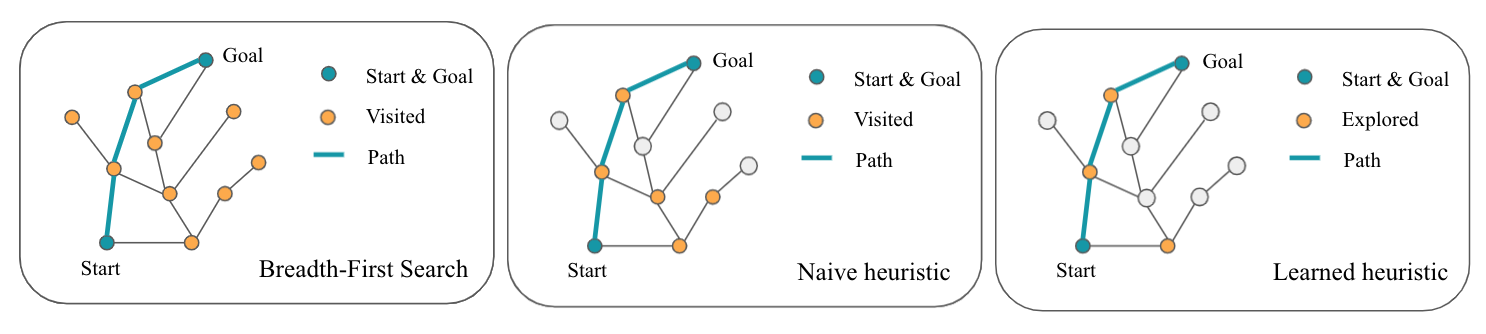
\includegraphics[width=0.9\textwidth]{figures/money_fig.png}
\caption{The goal is to navigate (find a path) from the start to the goal node. While BFS visits many nodes to find a start-to-goal path (left), one can use a heuristic based on the features of the nodes (e.g., Euclidean distance) on the graph to reduce the search effort (middle). We propose \alg to learn a tailored search heuristic for a given graph, capable of reducing the number of visited nodes even further by exploiting the inductive biases of the graph (right). }
\label{fig:money-fig}
\end{figure}

The search task can be formulated as a pathfinding problem on a graph, where given a graph, the task is to navigate and find a short feasible path from a start node to a goal node, while in the process visiting as few nodes as possible (Figure~\ref{fig:money-fig}). The most straightforward approach would be to launch a search algorithm such as breadth-first search (BFS) and iteratively expand the graph from the start node until it reaches the goal node. Since BFS does not harness any prior knowledge about the graph, it usually visits many nodes before reaching the goal, which is expensive in cases such as robotics where visiting nodes is costly. To visit fewer nodes during the search, one may use domain-specific information about the graph via a \textit{heuristic} function \cite{pearl1984heuristics}, which allows one to define a distance metric on graph nodes to prune directions that seem less promising to explore. Unfortunately, coming up with good search heuristics requires significant domain expertise and manual effort.
%, without straightforward ways to further refine proposed heuristics. 

While there has been significant progress in designing search heuristics, it remains a challenging problem. Classical approaches \cite{khalidi2020t, adabala2020multi} tend to hand-design search heuristics, which requires domain knowledge and a lot of trial and error. To alleviate this problem, there has been significant development in general-purpose search heuristics based on trading-off greedy expansions and novelty-based exploration \cite{xie2012planning, xie2014adding, lipovetzky2017best, teichteil2021boundary} or search problem simplifications \cite{bonet2001planning, zhu2003landmark, richter2010lama}. These approaches alleviate some of the common pitfalls of goal-directed heuristics, but we demonstrate that if possible, it is useful to learn domain-specific heuristics that can better exploit problem structure.

On the other hand, learning-based methods face a set of different challenges. Firstly, the data distribution is not i.i.d., as newly encountered graph nodes depend on past heuristic values, which means that supervised learning-based methods are not directly applicable. Secondly, heuristics should run fast, with ideally constant time complexity. Otherwise, the overall asymptotic time complexity of the search procedure could be increased. Finally, as the environment (search graph) sizes increase, reinforcement learning-based heuristic learning approaches tend to perform poorly \cite{bhardwaj2017learning}. State-of-the-art imitation learning-based methods can learn useful search heuristics \cite{bhardwaj2017learning}; however, these methods still rely on feature-engineering for a specific domain and do not generally guarantee a constant time complexity with respect to graph sizes.


\begin{figure}[h]
\centering
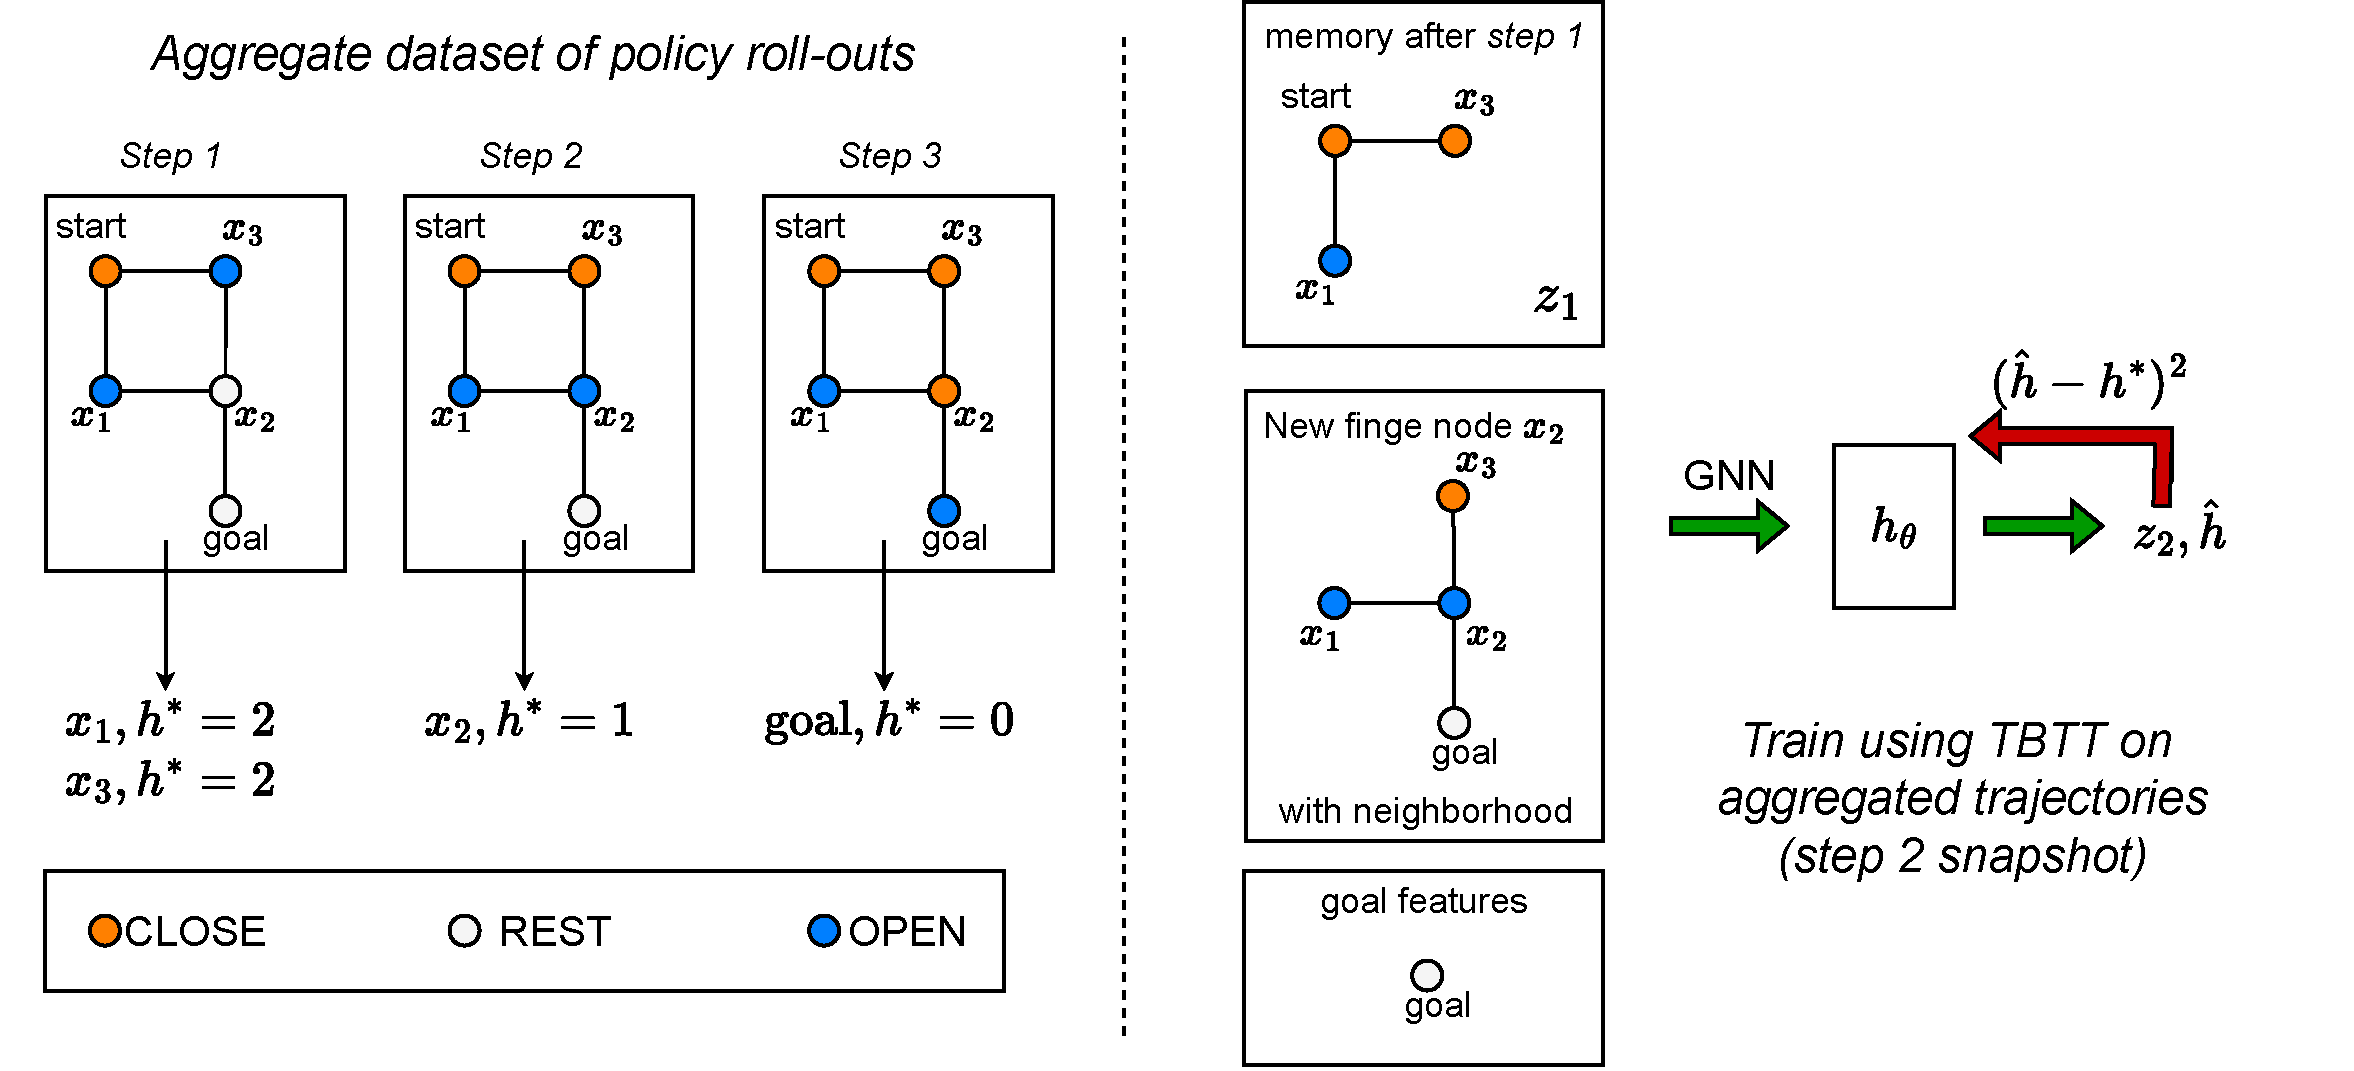
\includegraphics[width=0.9\textwidth]{figures/method_figure2.pdf}
\caption{Main components of \alg: On the left, using a greedy mixture policy induced by the current version of our parameterized heuristic $h_\theta$ and an oracle heuristic $h^*$ (i.e., a heuristic that correctly determines distances between nodes), we roll-out a search trajectory from the start node to the goal node. Each trajectory step contains a set of newly added fringe nodes with bounded random subsets of their 1-hop neighborhoods and their oracle ($h^*$) distances to the goal node. Trajectories are aggregated throughout the training procedure. On the right, we use truncated backpropagation through time on each collected trajectory to train $h_\theta$, where $\hat{h}$ is the predicted distance between $x_2$ and $x_g$, and $z_2$ is the updated state of the memory. Here, the memory captures the embedding of the graph visited so far.}
\label{fig:approach-high-level}
\end{figure}

%\jure{Here we say ``memory'', can we continue the sentence to explain what memory is. Something like: , which captures the graph visited so far.} \update{Added a short sentence at the end}
%\jure{Questions:\\
%-- what is "aggregate dataset"? So far we just explained that there is a graph, a start and a goal node. We need to explain what "aggregate dataset" is or change the label.\\
%-- can we use the concepts introduce in the main text in this figure as well.\\
%-- why do we label $x_{end}$? shouldn't we call it $x_{g}$. Let's use consistent terminology. Also $d_gt$ can we define it.\\
%-- Basically, if we use symbols in the figure, let's define them in the caption.}

%We formulate finding search heuristics as an optimization process, allowing practitioners to quickly find useful search heuristics. We illustrate this concept in Figure \ref{fig:money-fig}.


In this paper, we propose \textit{Path Heuristic with Imitation Learning} (\alg), a framework that extends the recent imitation learning-based heuristic search paradigm with a learnable \textit{explored graph memory}. This means that \alg learns a representation that allows it to capture the structure of the so far explored graph, so that it can then better select what node to explore next (Figure \ref{fig:approach-high-level}).  We train our approach to predict the node-to-goal distances ($h^{*}$ in Figure \ref{fig:approach-high-level}) of graph nodes during search. To train our memory module, which captures the explored graph, we use truncated backpropagation through time (TBTT) \cite{sutskever2013training}, where we utilize ground-truth node-to-goal distances as a supervision signal at each search step. Our TBTT procedure is embedded within an adaptation of the AggreVaTe imitation learning algorithm \cite{ross2014reinforcement}. \alg also includes a \textit{specialized graph neural network architecture}, which allows us to apply \alg to diverse graphs from different domains.

%\jure{Here we introduce many concepts: like ``explored graph'', ``memory module'', ``TBTT'', ``cost-to-go'', ... Can we please make sure to use these concepts in Fig 2 (have some part of the figure labeled using these labels.}

%Figure \ref{fig:approach-high-level} presents the high-level idea of our approach. 

We evaluate \alg on standard benchmark heuristic learning datasets (Section \ref{sec:experiments-grids}), diverse graph-based datasets from different domains (Section \ref{sec:experiments-diversity}), and practical UAV flight use cases (Section \ref{sec:experiments-drone}). Experiments demonstrate that \alg outperforms state-of-the-art heuristic learning methods up to $4 \times$. Further, \alg performs within $4.9 \%$ of an oracle in indoor drone planning scenarios, which is up to a $21.5 \%$ reduction compared with commonly used approaches. In practice, our contributions enable practitioners to quickly extract useful search heuristics from their graph datasets without any hand-engineering.
\section{Preliminaries}
\label{sec:prelims}
\xhdr{Graph search} Suppose that we are given an unweighted connected graph $\mathcal{G} = (\VS, \mathcal{E})$, where $\VS$ is a set of nodes, and $\mathcal{E}$ a corresponding set of edges. Further suppose that each node $i \in \VS$ has corresponding features $x_i \in \mathbb{R}^{D_v}$, and each edge $(i, j) \in \mathcal{E}$ has features $e_{ij} \in \mathbb{R}^{D_e}$. Assume that we are also given a start node $v_s \in \VS$ and a goal node $v_g \in \VS$. At any stage of our search algorithm, we can partition the nodes of our graph into three sets as $\VS = \text{CLOSE} \cup \text{OPEN} \cup \text{REST}$, where CLOSE are the nodes already explored,  $\text{OPEN}$ are candidate nodes for exploration (i.e., all nodes connected to any node in CLOSE, but not yet in CLOSE), and $\text{REST}$ is the rest of the graph. Each \textit{expansion} moves a node from $\text{OPEN}$ to CLOSE, and adds the neighbors of the given node from $\text{REST}$ to $\text{OPEN}$. We call the set of newly added fringe nodes $\VS_{new}$ at each search step.  At the start of the search procedure, $\text{CLOSE} = \{v_s\}$ and we expand the nodes until $v_g$ is encountered (i.e., until $v_g \in \text{CLOSE}$).

\xhdr{Greedy best-first search} We can perform \textit{greedy best-first search} using a greedy fringe expansion policy, such that we always expand the node $v \in \text{OPEN}$ that minimizes $h(v, v_g)$. Here, $h : \VS \times \VS \longrightarrow \mathbb{R}$ is a tailored heuristic function for a given use case. In our work, we are interested in learning a function $h$ that predicts shortest path lengths, this way minimizing $|\text{CLOSE}|$ in a \textit{greedy best-first search} regime.

%\update{Best-first should be clearer now - also organized this section a bit more}


%jure{We never define what a clairvoyant oracle is. Isn't oracle already optimal/supernatural/} \update{We decide to just use oracle for symbol brevity and it's easier to understand.}
\xhdr{Imitation of perfect heuristics} Partially observable Markov decision processes (POMDPs) are a suitable framework to describe the problem of learning search heuristics~\cite{bhardwaj2017learning}. We can have $s = (\text{CLOSE}, \text{OPEN}, \text{REST})$ as our state, an action $a \in \mathcal{A}$ corresponds to moving a node from $\text{OPEN}$ to CLOSE, and the observations $o \in \mathcal{O}$ are the features of newly included nodes in $\text{OPEN}$. Note that one could consider an MDP framework to learn heuristics, but the time complexity of operating on the whole state is in most cases prohibitive. We also define a history $\psi \in \Psi$ as a sequence of observations $\psi = o_1, o_2, o_3, ...$. Our work leverages the observation that using a heuristic function during greedy best-first search that correctly determines the length of the shortest path between fringe nodes and the goal node will also yield minimal $|\text{CLOSE}|$. For training, we adopt a perfect heuristic $h^{*}$, similar to \cite{bhardwaj2017learning}, which has full information about $s$ during search. Such oracle can provide ground-truth distances $h^{*}(s, v, v_g)$, where $v \in \text{OPEN}$. To conclude, we define a \textit{greedy best-first search policy} $\pi_{\theta}$ that uses a parameterized heuristic $h_{\theta}$ to expand nodes from $\text{OPEN}$ with minimal heuristic values. One could also directly use a POMDP solver for the above-described problem, but this approach is usually infeasible due to the dimensionality of the search state \cite{choudhury2017adaptive}.

%\update{Policy defined}

%Consider a partially observable Markov decision process (POMDP) defined by an 8-tuple $(S, A, R, P, \Omega, O, \gamma, \rho_0)$. In this POMDP definition, we have $S$ being a set of valid states, $A$ set of valid actions, $R : S \times A \longrightarrow \mathbb{R}$ the reward function, $P : S \times A \longrightarrow \mathcal{P}(S)$ the transition probability function, $\rho_0$ the initial state distribution, $\gamma \in [0, 1]$ the discount factor, $\Omega$ the set of observations, and $O : S \times A \longrightarrow \mathcal{P}(\Omega)$ a conditional observation probability function. We can also define a history $\psi \in \Psi$ as a sequence of observations $\psi = o_1, o_2, o_3, ...$. In general, our goal is to find an action policy $\pi(\cdot | \psi)$ that maximizes expected discounted rewards under the induced trajectory distribution. 

\section{Related Work}

\xhdr{General purpose heuristic design} There has been significant research in designing general-purpose heuristics for speeding up satisficing planning. The first set of approaches are based on simplifying the search problem for example using landmark heuristics \cite{bonet2001planning, richter2010lama}. The next set of approaches aim to include novelty-based exploration in greedy best-first search \cite{xie2012planning, xie2014adding, lipovetzky2017best, teichteil2021boundary}. The latter set of approaches showed state-of-the-art performance (best-first width search \cite{lipovetzky2017best, teichteil2021boundary}, BFWS) in numerous settings. We show that in domains where data is available, it can be more effective to incorporate a learned heuristic into a greedy best-first search procedure.


\xhdr{Learning heuristic search} There have been numerous previous works that attempt to learn search heuristics: Arfaee \etal \cite{arfaee2011learning} propose to improve heuristics iteratively, Virseda \etal  \cite{us2013learning} learn to combine heuristics to estimate graph node distances, Wilt \etal \cite{wilt2015building} and Garrett \etal \cite{garrett2016learning} propose to learn node rankings, Thayer \etal \cite{thayer2011learning} suggest to infer heuristics during a search, and Kim \etal \cite{KimA20} train a neural network to predict graph node distances. These methods generally do not consider the non-i.i.d. nature of heuristic search. Further, Bhardwaj \etal \cite{bhardwaj2017learning} propose \sail, where heuristic learning is framed as an imitation learning problem with cost-to-go oracles. The \sail heuristic uses hand-designed features tailored for obstacle avoidance, with a linear time-complexity in the number of explored grid nodes found to be colliding with an obstacle. Feature-engineering becomes more difficult as we attempt to learn heuristics on diverse graphs such as ones seen in Section \ref{sec:experiments-diversity}, where we may need expert knowledge. Further, heuristics that do not have a constant time complexity in the size of the graph \cite{bhardwaj2017learning, ariki2019fully, terasawa20203d, yonetani2020path, archetti2021neural} generally scale poorly with graph size and hence have constrained use cases. Recent approaches to learning heuristics include Retro* \cite{chen2020retro} by Chen \etal, where a heuristic is learned in the context of AND-OR search trees for chemical retrosynthetic planning. Our work focuses on a more general graph setting.

There has been significant progress on learning heuristics for NP-hard combinatorial optimization problems \cite{NIPS2017_d9896106, NEURIPS2018_8d3bba74, NEURIPS2020_49f85a9e}. Focusing on solving NP-hard problems allows these approaches to design algorithms that are often non-exact and have a relatively large computational budget. This is not the case for methods that focus on polynomial time search, where learning-based methods are bounded by the determinism and time complexity of classical algorithms such as greedy best-first search.



%Still, these heuristic learning methods, due to their time complexities, are impractical for the application in polynomial-time search problems, on which this work focuses.

%\textbf{\phil generally runs in $\mathcal{O}(1)$ per prediction without requiring any hand-engineering. We provide a comprehensive comparison with \sail in Section \ref{sec:experiments-grids}.}

%recent works by Ariki \etal \cite{ariki2019fully} and Teresawa \etal \cite{terasawa20203d} perform convolutions over full-graphs to infer their heuristic values, which  


\xhdr{Learning general purpose search} 
Learning general search policies is a very well-studied research area with a rich set of developments and applications. These include Monte Carlo Tree Search methods \cite{silver2010monte, guez2018learning}, implicit planning methods \cite{deac2020xlvin, karkus2017qmdp, tamar2016value}, and imagination-based planning approaches \cite{pascanu2017learning, weber2017imagination}. Learning search heuristics can be seen as a special case of \textit{general purpose search}, where the search problem is treated as a partially observable Markov decision process with restricted action evaluation (see Section \ref{sec:approach}), and with models running in $\mathcal{O}(1)$ to remain competitive time-complexity-wise on problems where best-first search performs well. \textit{General purpose search} methods do not take into account the above-mentioned constraints, which motivates the development of tailored approaches for learning heuristics \cite{ bhardwaj2017learning, chen2020retro}.

%\jure{I am not sure what precisely are we trying to say here and how does our method relate/differ from this} \update{The goal here was to answer the question of 'why not just use MCTS or something implicit like VIN'. I tried to rephrase the paragraph so that it is clear. I am also happy to drop this in case you think it is not necessary.}

\xhdr{Imitation learning} Our approach builds on prior work in imitation learning (IL) with cost-to-go oracles. Cost-to-go oracles have been incorporated in the context of IL in methods such as SEARN \cite{daume2009search}, AggreVaTe \cite{ross2014reinforcement}, LOLS \cite{chang2015learning}, AggrevaTeD \cite{sun2017deeply}, DART \cite{laskey2017dart}, and THOR \cite{sun2018truncated}. \sail \cite{bhardwaj2017learning} presents an AggreVaTe-based algorithm for learning heuristic search. We extend \sail by incorporating a recurrent $Q$-like function, in which sense our algorithm more closely resembles AggreVaTeD by Sun \etal \cite{sun2017deeply}. While a recurrent policy can be easily incorporated in AggreVaTeD, we cannot use a policy to evaluate actions. This is due to the fact that we would either have to evaluate all actions in a state, which is computationally infeasible, or we would have to give up on taking actions that are not in the most recent version of the search fringe, which would degrade the performance (see Section \ref{sec:approach}). %RNNs have been previously incorporated in SEARNN by Leblond \etal \cite{searnn} in the context of structured prediction, however we focus on imitation of cost-to-goal oracles. 

%nstead, we propose to use backpropagation through time on the roll-out phase of our algorithm, with cost-to-go supervision on each time step.
\section{Path Heuristic with Imitation Learning}
\label{sec:approach}

%\jure{Notice notation here is using $v_s$, $v_g$, where s is start and t is target. This is not consistent with introduction. Let's fix intro to use the same terminology.}

\xhdr{Training objective} With the aim of minimizing $|\text{CLOSE}|$ after search, our goal is to train a parameterized heuristic function $h_{\theta} : \Psi \times \VS \times \VS \longrightarrow \mathbb{R}$ to predict ground-truth node distances $h^{*}$ and use $h_\theta$ within a greedy best-first policy $\pi_\theta$ at test time.  More specifically, we assume access to a distribution over graphs $P_{\mathcal{G}}$, a start-goal node distribution $P_{v_{sg}}(\cdot \: | \: \mathcal{G})$, and a time horizon $T$. Moreover, we assume a joint state-history distribution $s, \psi \sim P_s(\cdot \: | \: \mathcal{G}, t, \pi_{\theta}, v_s, v_g)$, where $P_s$ represents the probability our search being in state $s$, at time $0 \leq t \leq T$ on graph $\mathcal{G}$ with pathfinding problem $(v_s, v_g)$, with a greedy best-first search policy $\pi_{\theta}$ using heuristic $h_{\theta}$. Hence, our goal can be summarized as minimizing the following objective:

\begin{equation}
    \label{eq:obj}
    \mathcal{L}(\theta) = \mathop{\EX}_{\substack{\mathcal{G} \sim P_{\mathcal{G}}, \\ (v_s, v_g) \sim P_{v_{sg}} \\ t \sim \mathcal{U}(0, ..., T), \\ s, \psi \sim P_s}}\big[\frac{1}{|\text{OPEN}|}\sum_{v \in \text{OPEN}} (h^{*}(s, v, v_g) - h_{\theta}(\psi, v, v_g))^{2} \big]
\end{equation}

Before we describe the algorithm that can be used to minimize $\mathcal{L}$, we rewrite $h_{\theta}$ to include a memory digest component ($z_t$), which represents an embedding of $\psi$ at time step $t$. Hence, $h_\theta$ becomes $h_{\theta} : \mathbb{R}^{d} \times \mathcal{O} \times \VS \times \VS \longrightarrow \mathbb{R}$, where $d$ is the dimensionality of our memory's embedding space. As opposed to previous methods \cite{bhardwaj2017learning}, $z_{t}$ allows us to \textit{automatically extract} relevant features for heuristic computations and concurrently \textit{reduce the computational complexity} of the heuristic function. Further, as shown in \cite{bhardwaj2017learning}, if we would use $h_{\theta}$ to evaluate all actions in a state (i.e., recalculate the heuristic values of all nodes in $\text{OPEN}$), we would need a squared reduction in the number of expanded nodes compared with BFS for \phil to bring performance benefits over BFS, which however may not be possible on all datasets. Hence, we constrain the heuristic only to evaluate new $\text{OPEN}$ nodes which we obtain after moving a node to $\text{CLOSE}$, calling the set of new fringe nodes $\VS_{new}$ after each expansion. In practice, the policy $\pi_{\theta}$  yields an algorithm equivalent to greedy best-first search, with the heuristic function replaced by $h_{\theta}$.

%\jure{This is the first time we define policy $\pi$ and it is unclear that it actually refers to our work PHIL}  \update{Should be clearer now: $\pi_{\theta}$ mentioned at the beginning of approach and in background}

\subsection{Learning algorithm \& architecture}
\label{sec:ila}

\begin{algorithm}[t]
	\caption{\phil --- Sequential Heuristic Training}\label{alg:il_alg}
	Obtain hyperparameters $T$, $\beta_{0}$, $N$, $m$, $t_\tau$;\\
	Initialize $\mathcal{D} \leftarrow \emptyset$, $h_{\theta_{1}}$; \\ \label{lst:line:}
	\For{$i = 1, \ldots, N$}
	{   Sample $\mathcal{G} \sim P_{\mathcal{G}}$; \\
	    Sample $v_s, v_g \sim P_{v_{sg}}$; \\
	    Set $\beta \leftarrow \beta_0^{i}$; \\
        Set mixture policy $\pi_{mix} \leftarrow (1 - \beta) * \pi_{\theta_{i}} + \beta  * \pi^{*}$; \\
	    Collect $m$ trajectories $\tau_{ij}$ as follows; \\
		\For{$j = 1,\ldots,m$}
		{   
			Sample $t \sim \mathcal{U}(0, ..., T - t_{\tau})$;\\
			Roll-in $t$ time steps of $\pi_{\theta_{i}}$ to obtain $z_t$ and new state $s_t = (\text{CLOSE}^{0}, \text{OPEN}^{0}, \text{REST}^{0})$; \\
			Roll-out trajectory $\tau_{ij}$ as follows;\\
			\For{$k = 1,\ldots, t_{\tau}$}
		    {   
    			Update $s_{t + k - 1}$ using $\pi_{mix}$ to get new state $s_{t+k}$ and new fringe state $\text{OPEN}^{k}$; \\
    			Obtain new fringe nodes $\VS_{new} = \text{OPEN}^{k} \setminus \text{OPEN}^{k-1}$; \\
    			Update trajectory $\tau_{ij} \leftarrow \tau_{ij} \cup \{(\VS_{new}, h^{*}(s_{t+k}, \VS_{new}, v_g))\}$; \\
	        }
		    Update dataset $\mathcal{D} \leftarrow \mathcal{D} \cup \{(\tau_{ij}, z_t)\}$ or $\mathcal{D} \cup \{(\tau_{ij}, 0)\}$; \\	
	    }
	    Train $h_{\theta_{i}}$ using TBTT on each $\tau \in \mathcal{D}$ to get $h_{\theta_{i+1}}$;\\  
	}
	\Return{best performing $h_{\theta_{i}}$ on validation};
\end{algorithm}


% Describe algo
\xhdr{Imitation learning algorithm} In Algorithm \ref{alg:il_alg}, we present the pseudo-code of the IL algorithm used to train our heuristic models (Figure \ref{fig:il-proc}). The high-level idea of our algorithm is that we aggregate trajectories of search traces (i.e., sequences of new fringe nodes) and use truncated backpropagation through time to optimize $h_{\theta}$ after each data-collection step. In particular, after sampling a graph $\mathcal{G}$ and a search problem  $v_s, v_g$, we use our greedy learned policy $\pi_\theta$ induced by $h_\theta$ to roll-in for $t \sim \mathcal{U}(0, \dots, T - t_{\tau})$ expansions, where $T$ is the episode time horizon, and $t_\tau$ is the roll-out length. From our roll-in, we obtain a new state $s = (\text{CLOSE}^{0}, \text{OPEN}^{0}, \text{REST}^{0})$, and an initial memory state $z_t$. After our roll-in, we roll-out for $t_{\tau}$ steps using our mixture policy $\pi_{mix}$, which is obtained by probabilistically blending $\pi_\theta$ and the greedy best-first policy induced by the oracle heuristic $\pi^{*}$. In a roll-out, we collect sequences of new fringe nodes, together with their ground-truth distances to the goal $v_g$, given by $h^{*}$.  Once the roll-out is complete, we append the obtained trajectory and the initial state for the following optimization using backpropagation through time. Further analysis on the trade-offs between using rolled-in states $z_t$ or zeroed-out states for training can be found in the supplementary material.

Note that we could also use supervised learning-based approaches to sample a fixed dataset of ($v_s$, $v_g$, $h^{*}(s, v_s, v_g)$) 3-tuples and train a model to predict node distances conditioned on their features. However, our experiments in Section \ref{sec:experiments} demonstrate that ignoring the non-i.i.d. nature of heuristic search negatively impacts model performance, with supervised learning-based methods performing up to $40 \times$ worse.


%\jure{As one is reading this, the question besomese, why not just sample some paths, and learn a MLP or GNN in the IID setting to predict the shortest path distance from current node to goal. It would be good to have a quick paragraph here discussing why this is not a good idea and a forward pointer to experiments/ablations which show that imitation learning gives x\% improvement over IID learning.} \update{Wrote a short paragraph about this.}

\begin{figure}[!htpb]
    \centering
    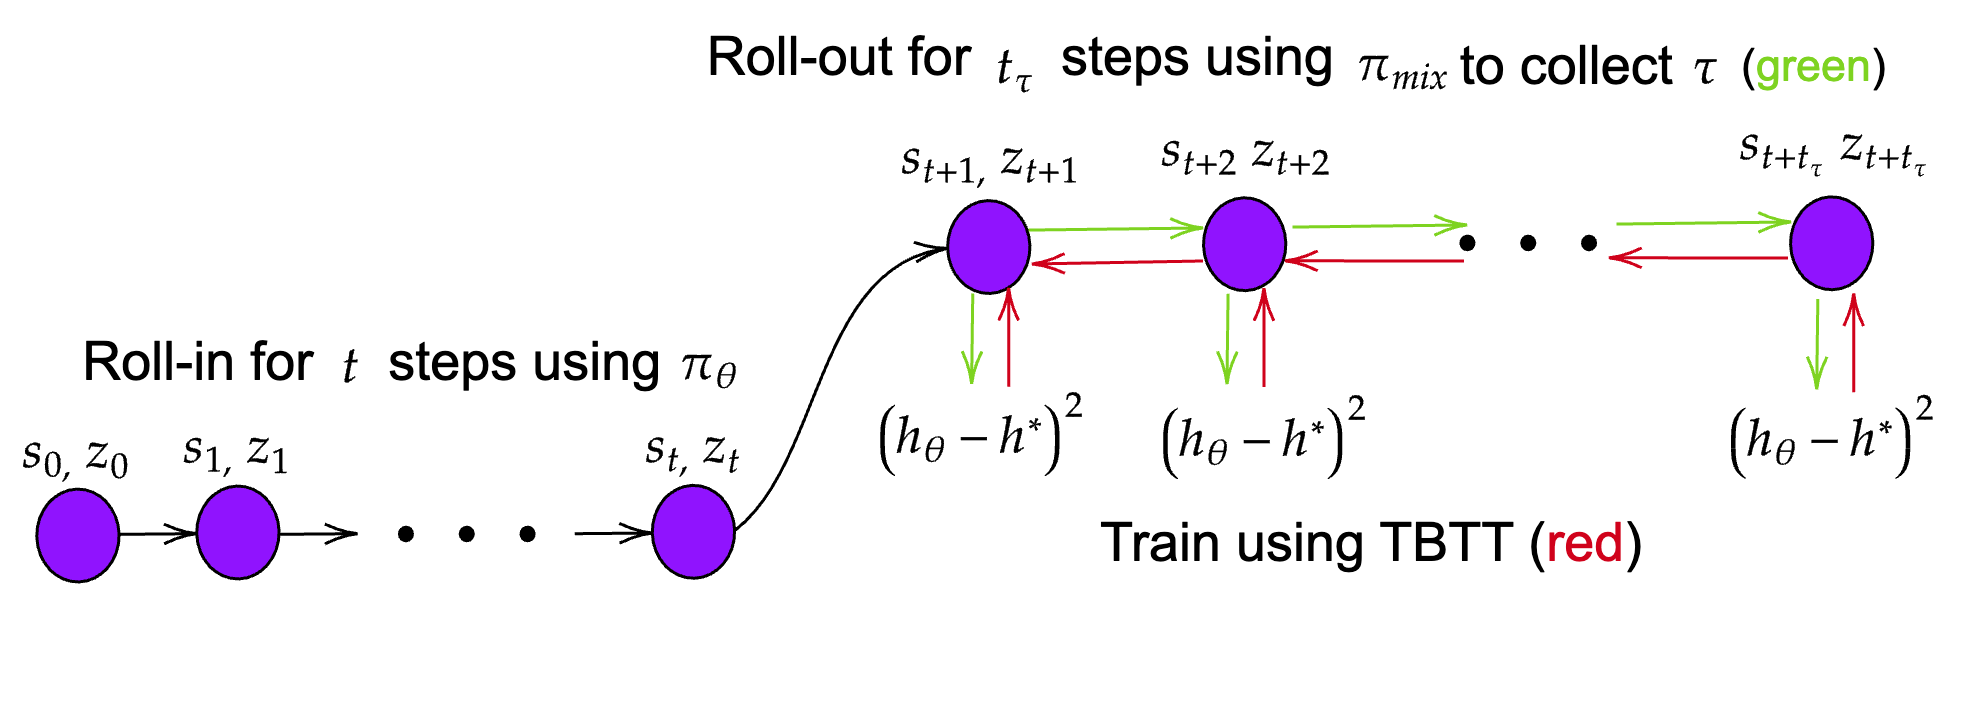
\includegraphics[width=0.9\textwidth]{figures/method_fig.png}
    \caption{This figure demonstrates the core idea behind our IL algorithm. We present the roll-in phase on the left-hand side, where our policy is rolled in for $t$ steps to obtain state $s_t$ and embedding $z_t$. On the right-hand side, we show the trajectory collection and training steps, where we aggregate the trajectory for downstream training (green) and use truncated backpropagation through time on the collected dataset (red).
    }
    \label{fig:il-proc}
    
\end{figure}

\begin{wrapfigure}[12]{R}{0.55\textwidth}
    \begin{algorithm}[H]
    	\caption{Heuristic func. ($h_\theta$) forward pass}\label{alg:htheta_alg}
    	 Obtain $x_i, x_j (j \in \mathcal{N}_i), e_{ij}, x_g$ $z_t$;\\
    	 $x_i \leftarrow f(x_i, x_g, D_{EUC}(x_i, x_g), D_{COS}(x_i, x_g)$);\\
     	 $x_j \leftarrow f(x_j, x_g, D_{EUC}(x_j, x_g), D_{COS}(x_j, x_g)$); \\
    
    	 $g_i \leftarrow \phi(x_i, \mathop{\oplus_{j \in \mathcal{N}_i}} \gamma(x_i, x_j, e_{ij}))$;\\
         $g^{\prime}_i, z_{i, t+1} \leftarrow \textsc{GRU}(g_i, z_t)$;\\
    	 $z_{t+1} \leftarrow \overline{z_{i, t+1}}$;\\ 
    	 $\hat{h}_i \leftarrow \textsc{MLP}(g^{\prime}_i, x_g);$\\
    	\Return{$\hat{h}_i ,z_{t+1}$};\\
    \end{algorithm}
\end{wrapfigure}


\textbf{Recurrent GNN architecture.} In each forward pass, $h_{\theta}$ obtains a set of new fringe nodes $\VS_{new}$, the goal node $v_g$, and the memory $z_t$ at time step $t$. We represent each node in $\VS_{new}$ using its features $x_{i} \in \mathbb{R}^{D_v}$, and likewise the goal node $v_g$ using its features $x_{g} \in \mathbb{R}^{D_v}$. Further, for each $i \in \VS_{new}$, we uniformly sample an $n \in \mathbb{N}_{\geq 0}$ bounded set of nodes present in the 1-hop neighborhood of $i$, calling this set $\mathcal{N}_i$, with $|\mathcal{N}_i| \leq n$. This sampling step produces a set of neighboring node features, where each $j \in \mathcal{N}_i$ has features $x_{j} \in \mathbb{R}^{D_v}$, and corresponding edge features $e_{ij} \in \mathbb{R}^{D_e}$.

%Further, for each $i \in \VS_{new}$, we uniformly sample up to $n \in \mathbb{N}_{\geq 0}$ nodes from the 1-hop neighborhood of $i$. This produces a bounded set of nodes $\mathcal{N}_i$, where $|\mathcal{N}_i| \leq n$, each $j \in \mathcal{N}_i$ has features $x_{j} \in \mathbb{R}^{D_v}$, and corresponding edge features $e_{ij} \in \mathbb{R}^{D_e}$.

%\jure{this header is confusing as for me ''model inference'' means inferring model parameters (and not a forward pass or prediction)}}
%\jure{It would be good to add a sentence here and describe what the goal is and remind people what i,j are and what y adn z are. Basically what are the inputs and what are the outputs} \update{Changed header name, explained what inputs/outputs are}.


\textbf{$h_{\theta}$ forward pass.}  Algorithm \ref{alg:htheta_alg} presents a single forward pass of $h_{\theta}$. The forward pass outputs predicted distances of the new fringe nodes to the goal $\hat{h}_i$, together with an updated memory digest $z_{t+1}$. In Algorithm \ref{alg:htheta_alg}, $f$, $\phi$, $\gamma$, $\textsc{GRU}$\cite{cho-etal-2014-learning}, $\textsc{MLP}$ are each parameterised differentiable functions, with $\phi, \gamma$ representing the \textit{update} and \textit{message} functions~\cite{gilmer2017neural} of a graph neural network, respectively.

In our forward pass, using the function $f$, we first project $x_i, x_j$ into a node embedding space, together with the goal features $x_g$, and their Euclidean ($D_{EUC}$) and cosine distances ($D_{COS}$). After that, using a $1$-layer GNN, we perform a single convolution over each $x_i$ and the corresponding neighborhood $\mathcal{N}_i$, to obtain $g_i$. Our graph convolution processing step allows us to easily incorporate edge features and work with variable sizes of $\mathcal{N}_i$. After the graph convolution, we apply the $\textsc{GRU}$ module over each embedding $g_i$ to obtain hidden states $z_{i, t+1}$, and new embeddings $g^{\prime}_i$. We compute the sample mean of $z_{i, t+1}$ for each node $i \in \VS_{new}$ to obtain a new hidden state $z_{t+1}$, and process $g^{\prime}_i$ with $x_g$ using an $\textsc{MLP}$ to compute the distances between the graph nodes. 

The intuitive explanation for using history embeddings is to address the partial observability of the problem. PHIL does not have access to the full graph because of time complexity concerns. The history embeddings provide a mechanism for keeping track of the belief over the full state of the graph during search. Further, the GNN allows for easily incorporating local neighborhoods and edge features.

\textbf{Permutation invariant $\VS_{new}$ embedding.} There is a trade-off between processing new fringe nodes in batch, as in Algorithm \ref{alg:htheta_alg}, and processing them sequentially. Namely, when we process the nodes in batch, we do not use the in-batch observations to predict batch node values, which means that $z_t$ is slightly outdated. On the other hand, in \phil, batch processing allows us to compute the heuristic values of all $v \in \VS_{new}$ in parallel on a GPU and preserves the memory's permutation invariance with respect to nodes in $\VS_{new}$. That is, because our observations are nodes \& edges of a graph, the respective observation ordering usually does not contain inductive biases useful for predictions, which means that we can apply a permutation invariant operator such as the mean of all new states $z_{i, t+1}$ to obtain an aggregated updated state. This approach provides additional scalability as we can process values in parallel and \phil does not have to infer permutation invariance in $ \VS_{new}$ from data.

\xhdr{Runtime complexity} Since $\forall i \in \VS_{new}: \: |\mathcal{N}_i| \leq n$, Algorithm \ref{alg:htheta_alg} together with neighborhood sampling runs in up to $nc_1 + (n+1)c_2$ operations per each node $i \in \VS_{new}$, which is $\mathcal{O}(1)$ with respect to the size of the graph. Here, $c_1$ is the maximal number of operations associated with evaluating a node, such as performing robot collision checks in dynamically constructed graphs, and $c_2$ is the maximal count of total model operations (e.g., $f$ \& $\gamma$ operations) on the node set $\{i\} \cup \mathcal{N}_i$. Note that for this analysis, we assume that $c_1$ is bounded. In general, we expect to learn a better search heuristic with increasing $n$, but in some use cases, $c_1$ may dominate overall complexity, which means the hyperparameter $n$ is helpful for practitioners to tune trade-offs between constant factors and search effort minimization.
\section{Experiments}
\label{sec:experiments}
In our experiments, we evaluate \phil both on benchmark heuristic learning datasets \cite{bhardwaj2017learning} (Section \ref{sec:experiments-grids}) as well on a diverse set of graph datasets (Section \ref{sec:experiments-diversity}). Finally, we show that \phil can be applied to efficient planning in the context of drone flight (Section \ref{sec:experiments-drone}). Our main goal is to assess how \phil compares to baseline methods in terms of necessary expansions before the goal node is reached.


\subsection{Heuristic search in grids}
\label{sec:experiments-grids}

\begin{wrapfigure}[13]{r}{0.3\textwidth}
  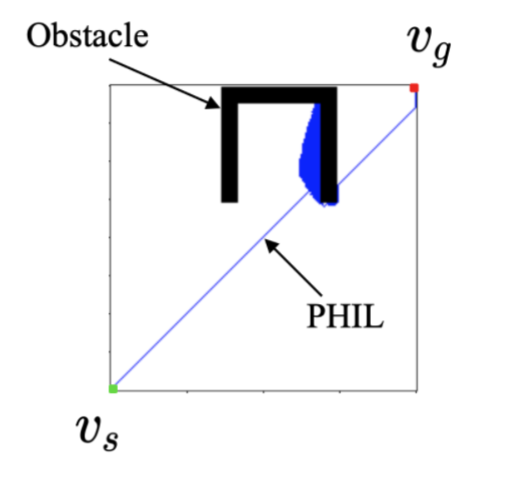
\includegraphics[width=\linewidth]{figures/local_minima.png}
    \caption{Example of \phil escaping local search minima.}
  \label{fig:local-min}
\end{wrapfigure}


In Section \ref{sec:experiments-grids}, we evaluate \phil on $8$, $200 \times 200$ 8-connected grid graph-based datasets by Bhardwaj \etal \cite{bhardwaj2017learning}. These datasets present challenging obstacle configurations for naive greedy planning heuristics, especially when $v_s$ is in the bottom-left of the grid, and $v_g$ in the top-right. Each dataset contains 200 training graphs, 70 validation graphs, and 100 test graphs. Example graphs from each dataset can be found in Table \ref{tab:table-1}.


We train \phil with a hyperparameter configuration of $T = 128$,  $t_{\tau} = 32$, $\beta_{0} = 0.7$, $n = 8$, and using rolled-in $z_t$ states as initial states for training. We use a 3-layer $\textsc{MLP}$ of width 128 with \textit{LeakyReLU} activations, followed by a DeeperGCN \cite{li2020deepergcn} graph convolution with \textit{softmax} aggregation. Our memory’s embedding dimensionality is $64$. The node features are 2D grid coordinates. Note that although using positional representations \cite{you2019position} might be useful for this search problem, it is not scalable as the graph size increases.

\begin{table*}[!htb]
\centering
\caption{The number of expanded graph nodes of \phil with respect to \sail. We can observe that out of all baselines, \sail performs best. \phil outperforms \sail by $58.5 \%$ on average over all datasets, with a maximal search effort reduction of $82.3 \%$ in the \textit{Gaps+Forest} dataset.}
\label{tab:table-1}
\resizebox{\columnwidth}{!}{%

\begin{tabular}{ccccccccccccccc} \toprule
 \textbf{Dataset} & \multicolumn{3}{c}{\textbf{Graph Examples}} & \textbf{\sail} & \textbf{SL} & \textbf{CEM} & \textbf{QL} & \textbf{$h_{euc}$} & \textbf{$h_{man}$} & \textbf{A*} & \textbf{MHA*} & \textbf{BFWS} & \textbf{Neural A*} & \textbf{\phil} \\ \midrule

Alternating gaps    & \frame{
\includegraphics[width=0.6cm, height=0.6cm]{figures/alt_1.png}} &  \frame{
\includegraphics[width=0.6cm, height=0.6cm]{figures/alt_2.png}}  &  \frame{
\includegraphics[width=0.6cm, height=0.6cm]{figures/alt_3.png}}   &0.039	&0.432& 0.042	& 1.000 & 1.000	&1.000	&1.000 & 1.000 & 0.34 &0.546 &\textbf{0.024}\\ 
Single Bugtrap       & \frame{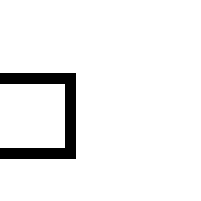
\includegraphics[width=0.6cm, height=0.6cm]{figures/sb1.png}} & \frame{
\includegraphics[width=0.6cm, height=0.6cm]{figures/sb2.png}}  & \frame{
\includegraphics[width=0.6cm, height=0.6cm]{figures/sb3.png}} 	& 0.158	& 0.214	& 0.057	& 1.000	&0.184	&0.192	&1.000	&0.286 & 0.099 &0.394 & 
\textbf{0.077} \\ 
Shifting gaps       & \frame{
\includegraphics[width=0.6cm, height=0.6cm]{figures/sg1.png}}  & \frame{
\includegraphics[width=0.6cm, height=0.6cm]{figures/sg2.png}}  & \frame{
\includegraphics[width=0.6cm, height=0.6cm]{figures/sg3.png}}  &0.104	&0.464	&1.000	&1.000	&0.506	&0.589	&1.000	&0.804 & 0.206 &0.563 &\textbf{0.027} \\
Forest              & \frame{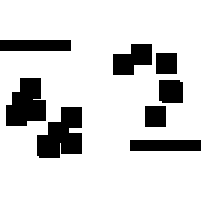
\includegraphics[width=0.6cm, height=0.6cm]{figures/f_1.png}}  & \frame{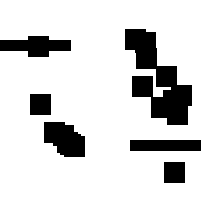
\includegraphics[width=0.6cm, height=0.6cm]{figures/f2.png}}  &  \frame{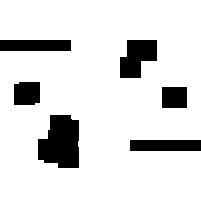
\includegraphics[width=0.6cm, height=0.6cm]{figures/f3.png}}   & 0.036 &0.043	&0.048	&0.121	&0.041	&0.043	&1.000	&0.075 & 0.039  &0.399 & \textbf{0.027}\\
Bugtrap+Forest      & \frame{
\includegraphics[width=0.6cm, height=0.6cm]{figures/bf_1.png}}  & \frame{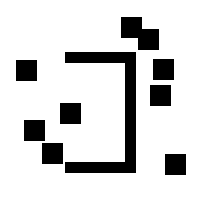
\includegraphics[width=0.6cm, height=0.6cm]{figures/bf_2.png}}  &  \frame{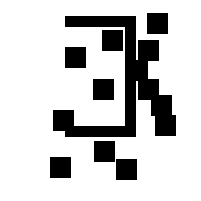
\includegraphics[width=0.6cm, height=0.6cm]{figures/bf_3.png}}  	&0.147	&0.384	&0.182	&1.000	&0.410	&0.337	&1.000	&3.177 & 0.149 &0.651 &\textbf{0.135} \\
Gaps+Forest         &\frame{ 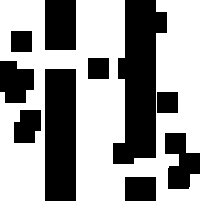
\includegraphics[width=0.6cm, height=0.6cm]{figures/gf1.png}}  & \frame{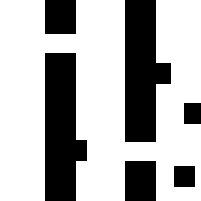
\includegraphics[width=0.6cm, height=0.6cm]{figures/gf2.png}}  & \frame{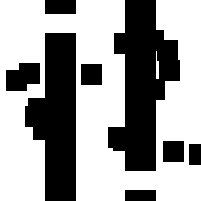
\includegraphics[width=0.6cm, height=0.6cm]{figures/gf3.png}}    	&0.221	&1.000	&1.000	&1.000	&1.000	&1.000	&1.000	&1.000 & 0.401 & 0.580 &\textbf{0.039} \\
Mazes               & \frame{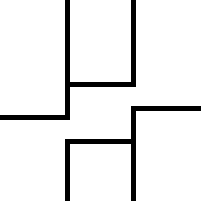
\includegraphics[width=0.6cm, height=0.6cm]{figures/m1.png}}  & \frame{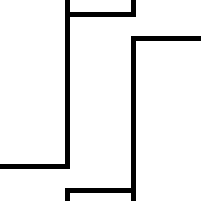
\includegraphics[width=0.6cm, height=0.6cm]{figures/m2.png}}  & \frame{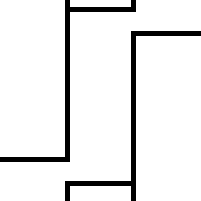
\includegraphics[width=0.6cm, height=0.6cm]{figures/m3.png}} 	&0.103	&0.238	&0.479	&0.399	&0.185	&0.171	&1.000	&0.279 & 0.095 &1.000 &\textbf{0.069}\\
Multiple Bugtraps   & \frame{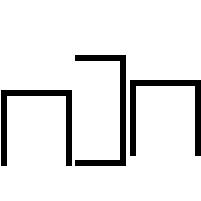
\includegraphics[width=0.6cm, height=0.6cm]{figures/mb1.png}}  & \frame{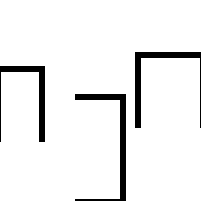
\includegraphics[width=0.6cm, height=0.6cm]{figures/mb2.png}}  & \frame{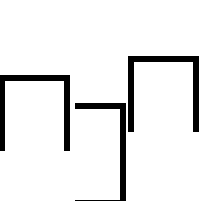
\includegraphics[width=0.6cm, height=0.6cm]{figures/mb3.png}} 	&0.479	&0.480	&1.000	&0.835	&0.648	&0.617	&1.000	&0.876 &0.169 &0.331 & \textbf{0.136}  \\ \bottomrule

% Alternating gaps    & \frame{
\includegraphics[width=0.6cm, height=0.6cm]{figures/alt_1.png}} &  \frame{
\includegraphics[width=0.6cm, height=0.6cm]{figures/alt_2.png}}  &  \frame{
\includegraphics[width=0.6cm, height=0.6cm]{figures/alt_3.png}}   &1.000	&11.077	&1.077	&25.641	&25.641	&25.641	&25.641	&25.641 & 8.718 & &\textbf{0.615}\\ 
% Single Bugtrap       & \frame{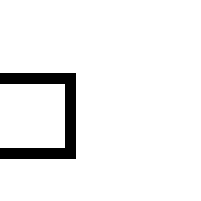
\includegraphics[width=0.6cm, height=0.6cm]{figures/sb1.png}} & \frame{
\includegraphics[width=0.6cm, height=0.6cm]{figures/sb2.png}}  & \frame{
\includegraphics[width=0.6cm, height=0.6cm]{figures/sb3.png}} 	&1.000	&1.354	&\textbf{0.361}	&6.329	&1.165	&1.215	&6.329	&1.772 & 0.625 & & 0.544 \\ 
% Shifting gaps       & \frame{
\includegraphics[width=0.6cm, height=0.6cm]{figures/sg1.png}}  & \frame{
\includegraphics[width=0.6cm, height=0.6cm]{figures/sg2.png}}  & \frame{
\includegraphics[width=0.6cm, height=0.6cm]{figures/sg3.png}}      &1.000	&4.462	&9.615	&9.615	&4.865	&5.663	&9.615	&7.731 & 1.982 & &\textbf{0.260} \\
% Forest              & \frame{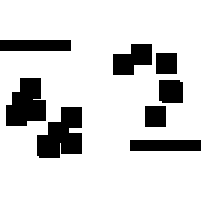
\includegraphics[width=0.6cm, height=0.6cm]{figures/f_1.png}}  & \frame{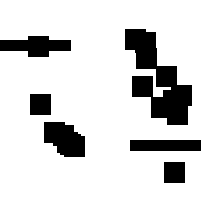
\includegraphics[width=0.6cm, height=0.6cm]{figures/f2.png}}  &  \frame{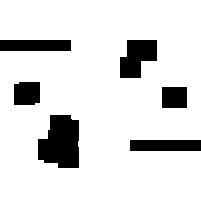
\includegraphics[width=0.6cm, height=0.6cm]{figures/f3.png}}             &1.000	&1.194	&1.333	&3.361	&1.139	&1.194	&27.778	&2.083 & 1.078 & & \textbf{0.778}\\
% Bugtrap+Forest      & \frame{
\includegraphics[width=0.6cm, height=0.6cm]{figures/bf_1.png}}  & \frame{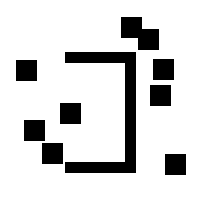
\includegraphics[width=0.6cm, height=0.6cm]{figures/bf_2.png}}  &  \frame{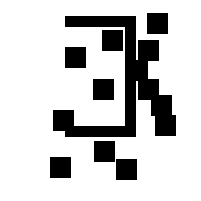
\includegraphics[width=0.6cm, height=0.6cm]{figures/bf_3.png}}  	&1.000	&2.612	&1.238	&6.803	&2.789	&2.293	&6.803	&3.177 & 1.011 & &\textbf{0.810} \\
% Gaps+Forest         &\frame{ 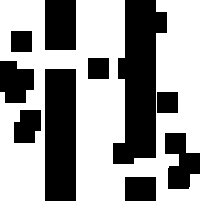
\includegraphics[width=0.6cm, height=0.6cm]{figures/gf1.png}}  & \frame{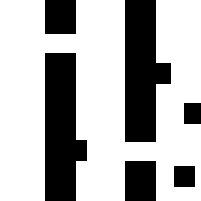
\includegraphics[width=0.6cm, height=0.6cm]{figures/gf2.png}}  & \frame{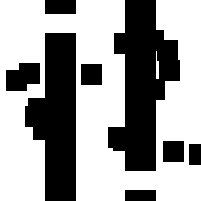
\includegraphics[width=0.6cm, height=0.6cm]{figures/gf3.png}}    	&1.000	&4.525	&4.525	&4.525	&4.525	&4.525	&4.525	&4.525 & 1.813 & &\textbf{0.213} \\
% Mazes               & \frame{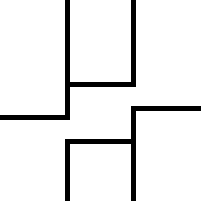
\includegraphics[width=0.6cm, height=0.6cm]{figures/m1.png}}  & \frame{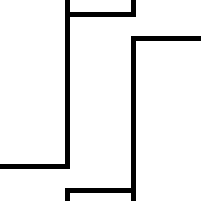
\includegraphics[width=0.6cm, height=0.6cm]{figures/m2.png}}  & \frame{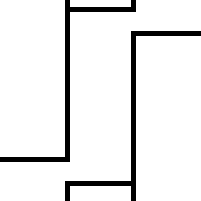
\includegraphics[width=0.6cm, height=0.6cm]{figures/m3.png}} 	&1.000	&2.311	&4.650	&3.874	&1.796	&1.660	&9.709	&2.709 & 0.921 & &\textbf{0.495}\\
% Multiple Bugtraps   & \frame{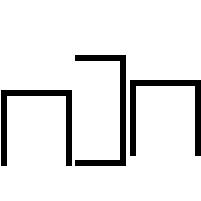
\includegraphics[width=0.6cm, height=0.6cm]{figures/mb1.png}}  & \frame{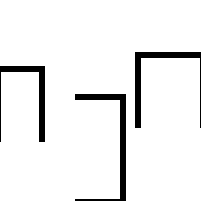
\includegraphics[width=0.6cm, height=0.6cm]{figures/mb2.png}}  & \frame{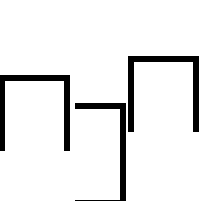
\includegraphics[width=0.6cm, height=0.6cm]{figures/mb3.png}} 	&1.000	&1.002	&2.088	&1.743	&1.353	&1.288	&2.088	&1.829 &0.353 & & \textbf{0.382}  \\ \bottomrule
\end{tabular}
}
\end{table*}

%\jure{Could we add squares/boxes around Graph Examples (as in Fig 4). I think then it will be much clearer that these are same things as in Fig 4).}
%\jure{Caption: Rather than discussing the baselines let's discuss performance and point out interesting observations. For example: ``Out of all baselines \sail performs best, while PHIL performs X\% better than \sail on average.'' Let's say something like this.} \update{boxes and quantified observations added}

\textbf{Discussion.} As we can see in Table \ref{tab:table-1}, \phil outperforms the best baseline (\textit{\sail}) on all datasets, with an average reduction of explored nodes before $v_g$ is found of $58.5 \%$.
%Even with \textit{CEM} performing better than \phil on \textit{Single Bugtrap}, \phil reduces the necessary search effort compared with the best baseline on each dataset by \michal{$40.8 \%$} on average.
Qualitatively, observing Figure \ref{fig:sail-comparison}, we can attribute these results to \phil's ability to \textbf{reduce the redundancy in explored nodes} during a search. Further, \phil is also \textbf{capable of escaping local minima}, which is illustrated in Figure \ref{fig:local-min}. However, note that we occasionally observe failure cases in practice, where \phil gets stuck in a bug trap-like structure.

\xhdr{Runtime \& convergence speed} \phil converges in up to $N = 36$ iterations, with $m = 1, t_\tau = 32$ (i.e., after observing less than $N * t_\tau * max(|\VS_{new}|) \approx 9,216$ shortest path distances, where we take $max(|\VS_{new}|) = 8$ as the maximal size of $\VS_{new}$). According to figures reported in \cite{bhardwaj2017learning}, this is approximately $5\times$ less data than it takes for \sail to converge.
%Although neither the \sail or \phil code-bases were optimized for runtime speed, we found that our implementation of \phil runs about $7 \times$ faster than the publicly available implementation of \sail on the \textit{Gaps+Forest} dataset.


%\jure{Same here, can we quantify performance: PHIL explores X\% less nodes on average than the second best method, Sail} \update{Should be better quantified \& more optimistic}
% \setlength{\framerule}{1pt}%

\begin{figure*}[h!]
    \centering
    \begin{adjustbox}{minipage=\linewidth,scale=0.9}

    \begin{subfigure}[t]{0.45\textwidth}
         \raisebox{-\height}{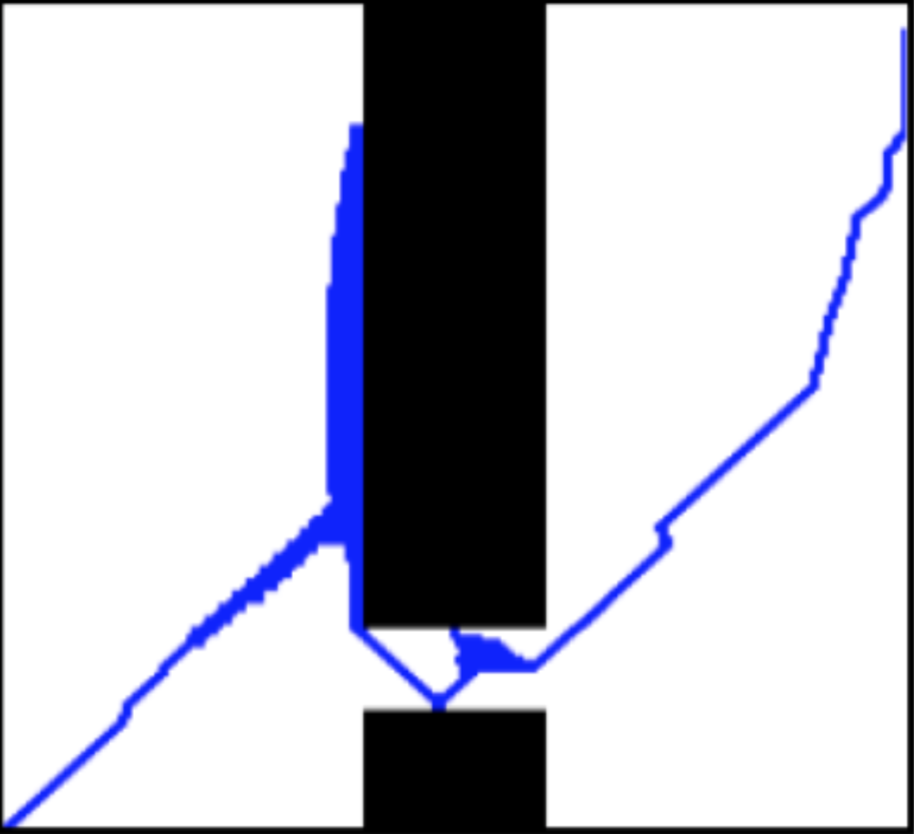
\includegraphics[width=0.49\textwidth,height=0.49\textwidth]{figures/c1_sail.png}}
         \raisebox{-\height}{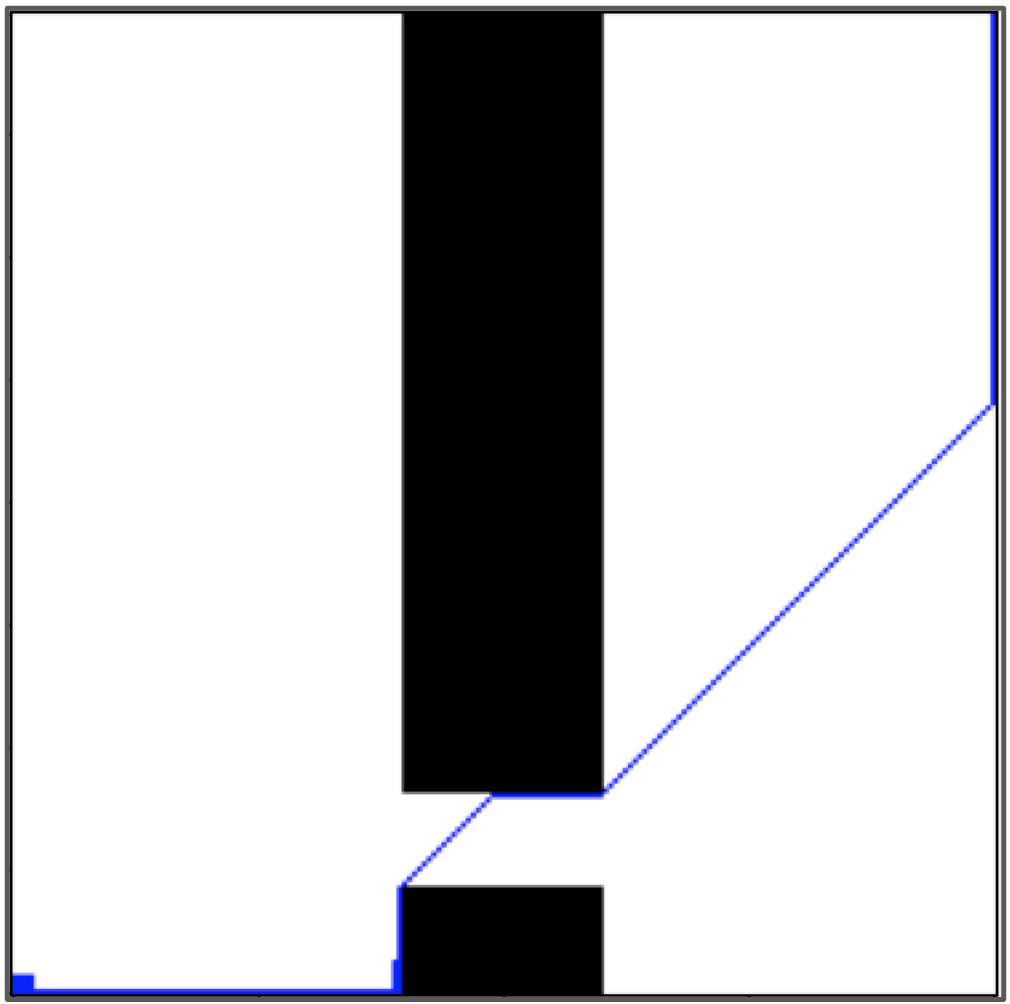
\includegraphics[width=0.49\textwidth,height=0.49\textwidth]{figures/c1.png}}%
         \label{fig:one-a}
    \caption{Shifting gaps (\sail left, \phil right)}
    \end{subfigure}
    \hfill
    \begin{subfigure}[t]{0.45\textwidth}
         \raisebox{-\height}{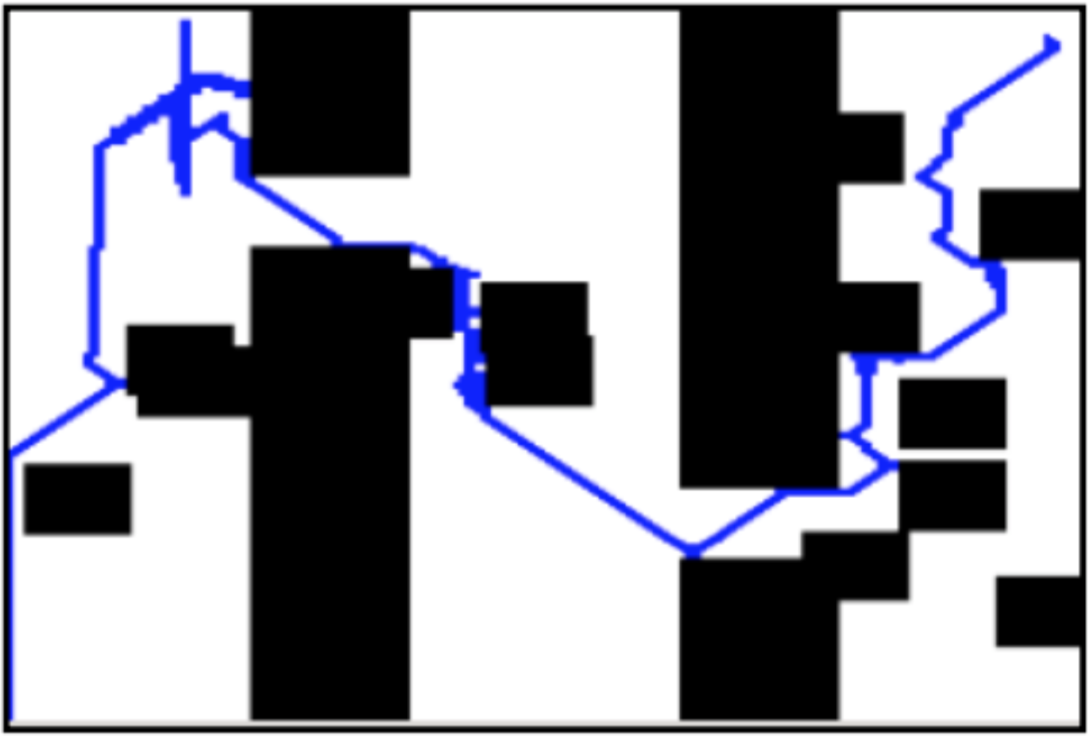
\includegraphics[width=0.49\textwidth,height=0.49\textwidth]{figures/c2_sail.png}}
         \raisebox{-\height}{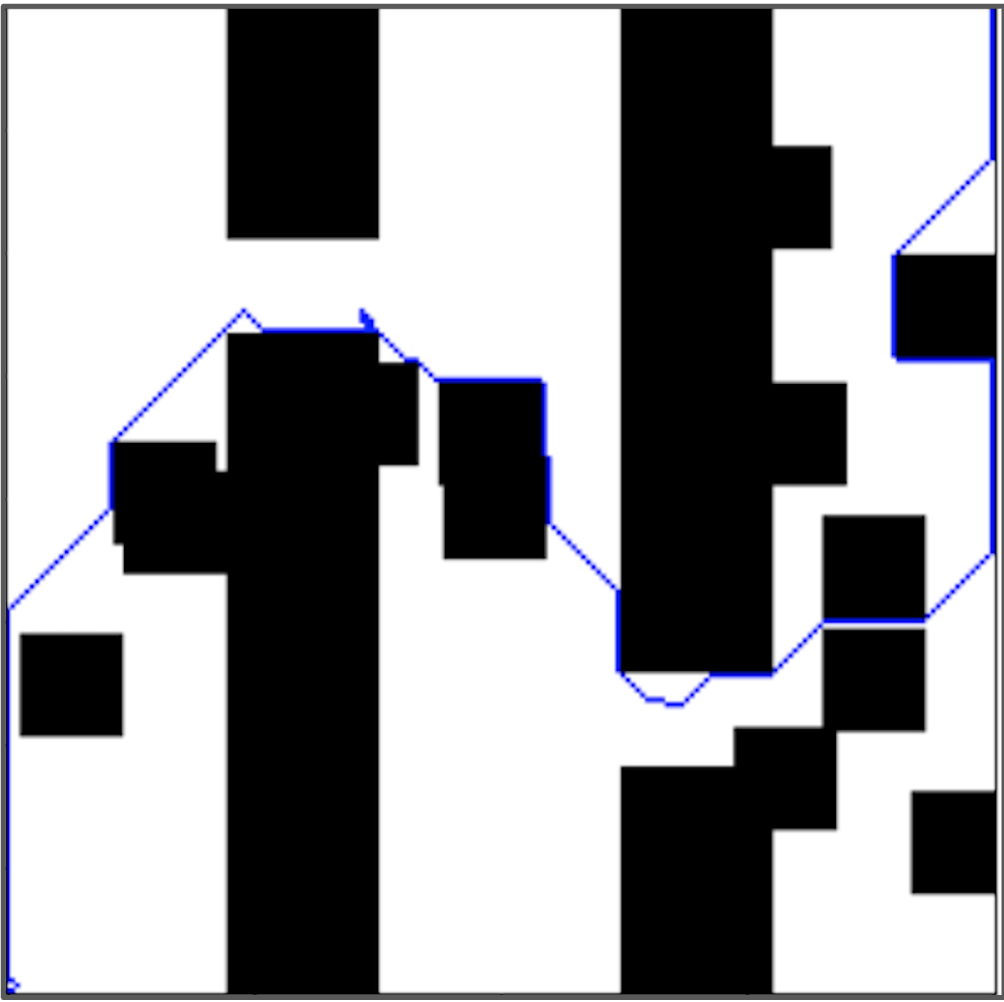
\includegraphics[width=0.49\textwidth,height=0.49\textwidth]{figures/c2.png}}%
    \caption{Gaps+Forest (\sail left, \phil right)}
    \end{subfigure}
    %%%%%%%%%%%%%%%%%%%%%%%%%%%%%%%%%%%%second row
    \begin{subfigure}[t]{0.45\textwidth}
        \raisebox{-\height}{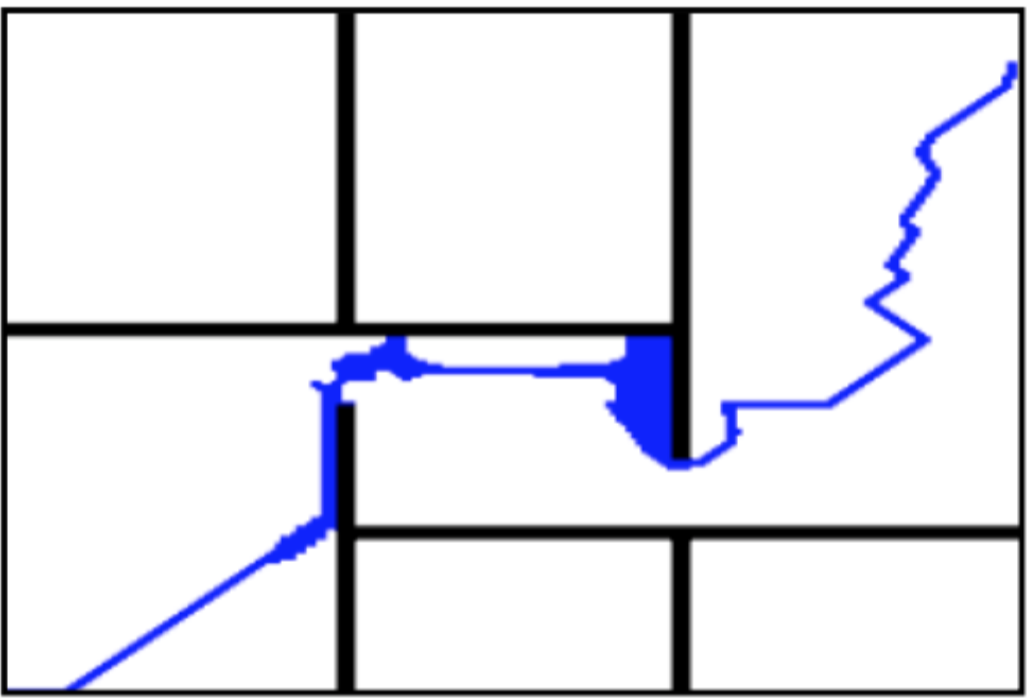
\includegraphics[width=0.49\textwidth,height=0.49\textwidth]{figures/c3_sail.png}}
        \raisebox{-\height}{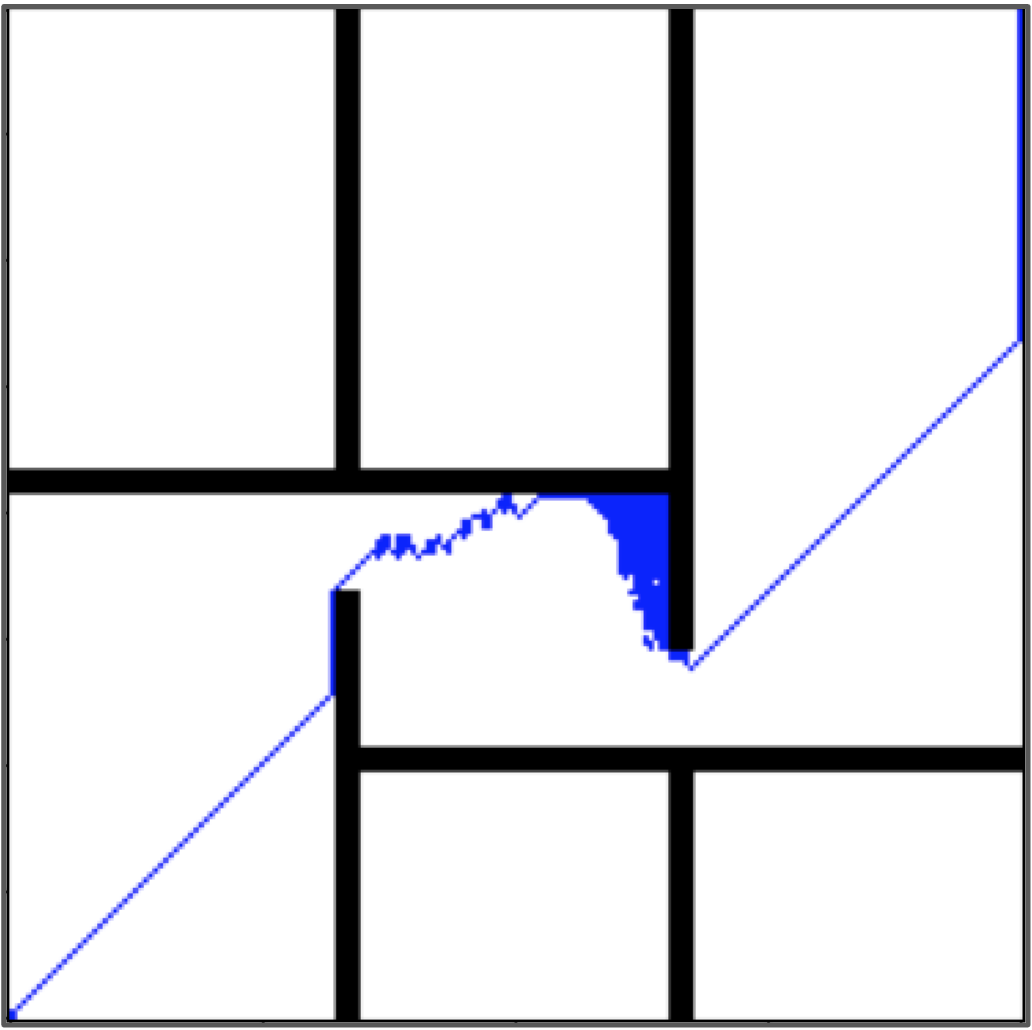
\includegraphics[width=0.49\textwidth,height=0.49\textwidth]{figures/c3.png}}%
    \caption{Mazes (\sail left, \phil right)}
    \end{subfigure}
    \hfill
    \begin{subfigure}[t]{0.45\textwidth}
          \raisebox{-\height}{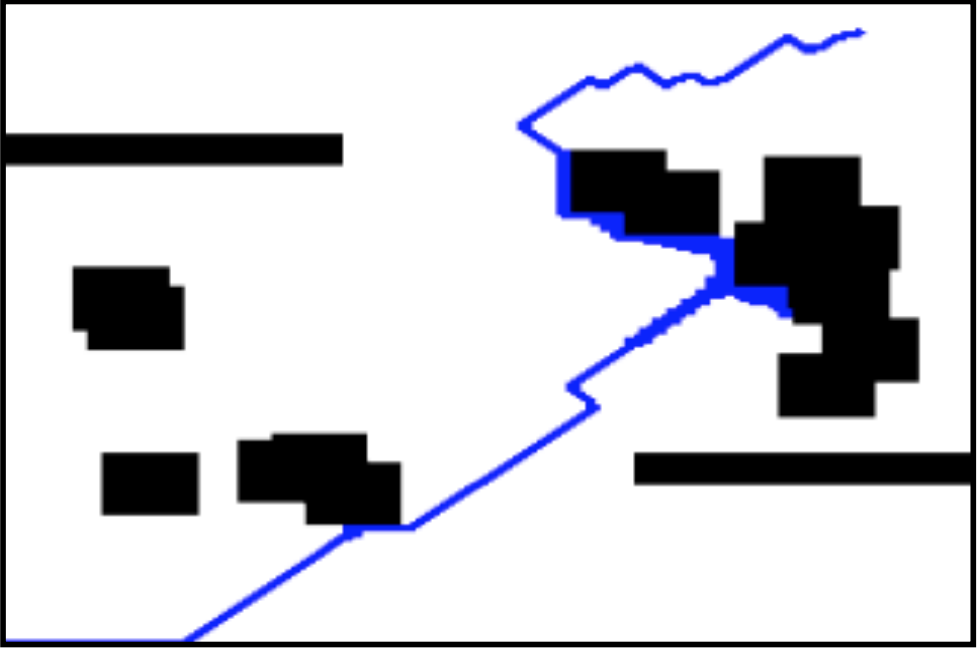
\includegraphics[width=0.49\textwidth,height=0.49\textwidth]{figures/c4_sail.png}}
          \raisebox{-\height}{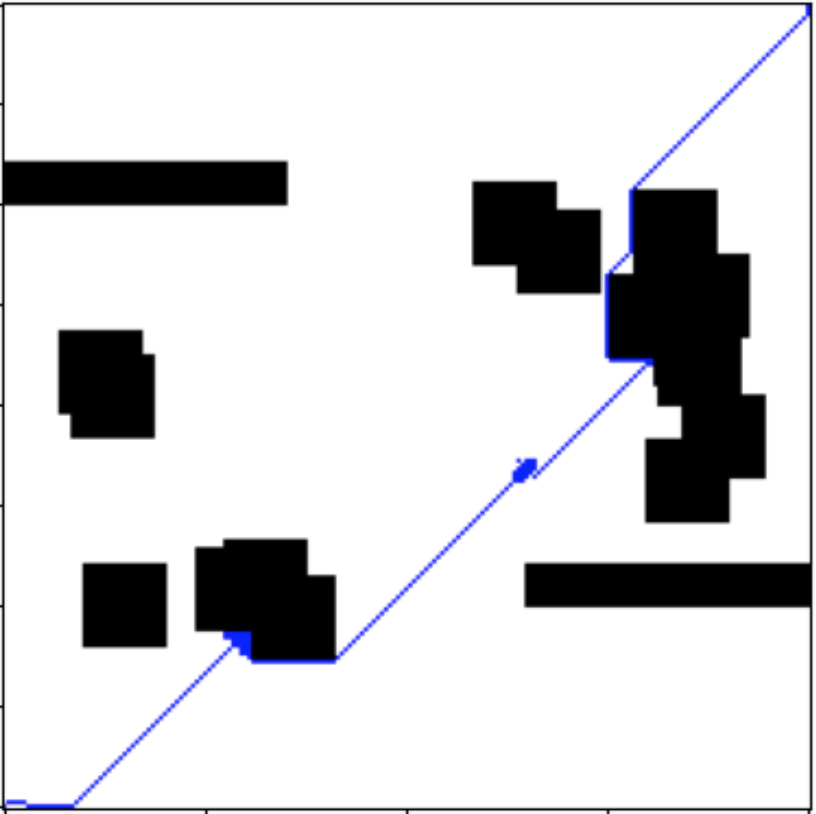
\includegraphics[width=0.49\textwidth,height=0.49\textwidth]{figures/c4.png}}%
    \caption{Forest (\sail left, \phil right)}
    \end{subfigure}
    \end{adjustbox}
    \caption{In each image pair of this figure, we provide a qualitative comparison with the \sail method. In particular, we show comparisons on the \textit{Shifting gaps}, \textit{Gaps+Forest}, \textit{Mazes}, and \textit{Forest} datasets. We can observe that \phil (right) learns the appropriate heuristics for the given dataset and makes fewer redundant expansions than \sail (left).
    %\jure{there seem to be a bug in the figure. I thought that we show the same graph but a different path.} \update{Bug should be fixed}
    } 
    \label{fig:sail-comparison}
\end{figure*}

\subsection{Search in real-life graphs of different structures}
\label{sec:experiments-diversity}

In this experiment, our goal is to demonstrate the general applicability of \phil to various graphs. We train \phil on $4$ different groups of graph datasets: citation networks, biological networks, abstract syntax trees (ASTs), and road networks. We use the same graph for citation networks and road networks for training and evaluation, and we use $100$ random $v_s, v_g$ pairs for testing. In the case of biological networks and ASTs, we usually have train/validation/test splits of $80/10/10$, and in the case of the OGB \cite{hu2020open} datasets, we use the provided splits.


\begin{table*}[!htb]
\centering
\caption{Comparison of \phil with baseline approaches on $4$ groups of datasets: citation networks, biological networks, abstract syntax trees, and road networks. "$-$" denotes being out of a 4-day's training time limit. We can observe that, on average across all datasets, \phil outperforms the best baseline per dataset by $13.4 \%$. Discounting the OGBG datasets, this number becomes $19.5 \%$.}
\label{tab:table-2}
\resizebox{\columnwidth}{!}{

\begin{tabular}{c|c|ccc|ccccccc} 
\toprule
& \textbf{Dataset} &\textbf{$|\mathcal{D}|$} &\textbf{$\bar{|\VS|}$} &\textbf{$\bar{|\mathcal{E}|}$}  & \textbf{SL} &\textbf{A*} &$h_{euc}$ &\textbf{BFS} & \textbf{\sail} & \textbf{BFWS} &\textbf{\phil} \\ \midrule
\multirow{5}{*}{Citation Networks} &Cora (Sen \etal \cite{sen2008collective}) &1 &2,708 &5,429 &2.201	&2.067	&1.000	&4.001 & 0.669 &1.378    &\textbf{0.475} \\ 
&PubMed (Sen \etal \cite{sen2008collective}))   &1 &19,717 &44,338            &2.157 &2.983	&1.000	& 3.853 & 1.196 &  1.000& \textbf{0.745}  \\ 
&CiteSeer (Sen \etal \cite{sen2008collective})) &1 &3,327 &4,732            &1.636 &1.487	&1.000	&2.190 & 1.062     &0.951  &\textbf{0.599}\\
&Coauthor (cs) (Schur \etal \cite{shchur2018pitfalls}) &1 &18,333 &81,894       &1.571	&1.069	&1.000	&2.820 & 1.941 &    1.026 &\textbf{0.835}\\
&Coauthor (physics) (Schur \etal \cite{shchur2018pitfalls}) &1 &34,493 &247,962  &4.076	&1.081	&1.000	&4.523 & $-$ & 1.012 &\textbf{0.964} \\ \midrule
\multirow{4}{*}{Biological Networks} &OGBG-Molhiv  (Hu \etal \cite{hu2020open}) &41,127 &25.5	&27.5  &1.086 &1.065 &\textbf{1.000} & 1.267 & 1.104 & 1.146 & 1.016  \\
&PPI (Zitnik \etal \cite{zitnik2017predicting})         &24 &2,372.67 &34,113.16 &0.772 &0.831 &1.000 &5.618 & 1.746 & 3.941 &\textbf{0.658}\\
&Proteins (Full) (Morris \etal \cite{morris2020tudataset})  &1,113 &39.06 &72.82 &0.995 &0.997 &1.000 &2.645 & 0.891 & 0.966 &\textbf{0.831}\\
&Enzymes (Morris \etal \cite{morris2020tudataset})            &600 &32.63 &62.14 &1.073	&1.007 &1.000 &1.358 & 1.036 & 0.992 &\textbf{0.757}\\ \midrule
\multirow{1}{*}{ASTs} &OGBG-Code2 (Hu \etal \cite{hu2020open}) &452,741 &125.2 &124.2  	&1.196  &1.013	&1.000	&1.267 & 1.029 & \textbf{0.817} & 1.219 \\ \midrule
\multirow{2}{*}{Road Networks} &OSMnx - Modena (Boeing \cite{boeing2017osmnx}) &1 &29,324 &38,309  &2.904 	&3.085	&1.000	&3.493 & 1.182 &0.997&\textbf{0.489}\\ 
&OSMnx - New York (Boeing \cite{boeing2017osmnx}) &1 &54,128 &89,618 & 39.424  &36.529	&1.000	&63.352 & 1.583&1.013 &\textbf{0.962}\\ 
\bottomrule
\end{tabular}
}
\end{table*}


%\jure{Let's add a sentence commenting on performance, let's quantify it.\\
%Also, can we add 2 more columns---size of the graph (nodes, edges).\\
%Call "city networks" "road networks".
%} \update{Added dataset stats and quantified results}

Similarly as in Section \ref{sec:experiments-grids}, our $\textsc{MLP}$ has four layers of width $128$ with \textit{LeakyReLU} activations and we use a DeeperGCN~\cite{li2020deepergcn} graph convolution with \textit{softmax} aggregation. The utilized node and edge features are the provided features in each dataset, except for a few minor modifications. We train an $\textsc{MLP}$ of depth $5$ and width $256$ using supervised learning (SL) for our learning-based baseline method. 

%Our classical baselines are greedy best-first search ($h_{euc}$) and A* with a euclidean distance heuristic on the node features and breadth-first search (BFS). In Table \ref{tab:table-2}, we report the ratio of explored nodes with respect to $h_{euc}$ after search.

\xhdr{Discussion} The results presented in Table \ref{tab:table-2} suggest that \phil can learn superior search heuristics compared with baseline methods, outperforming top baselines per dataset in terms of visited nodes during a search by $13.4 \%$ on average. Two datasets where \phil fell short compared to other baselines are the \textit{OGBG-Molhiv} and \textit{OGBG-Code2} datasets. The \textit{OGBG-Code2} dataset adopts a \textit{project split} \cite{allamanis2019adverse} and OGBG-Mohliv adopts a \textit{scaffold split} \cite{wu2018moleculenet}, both of which ensure that graphs of different structure are present in the training \& test sets. Although \phil improved upon uninformed search (BFS) in the OGB datasets, structural graph consistency is explicitly discouraged in the above-mentioned OGBG splits. Without the OGBG datasets, \phil improves on the top baselines per dataset by $19.5 \%$ on average, and upon the Euclidean node feature heuristic ($h_{euc}$) by $20.4 \%$. Note that we trained \phil up to $N = 60$ iterations, which means that it only encountered a small subset of the pathfinding problems in the single graph setting, which means that \phil had to generalize to learn useful heuristics. Even in Cora, the $|\mathcal{D}| = 1$ dataset with least number of nodes, \phil observed roughly $6,000$ node distances during training, which is less than $0.2 \%$ of total distances in the Cora graph.

%The \textit{OGBG-Molhiv} and \textit{OGBG-Code2} datasets contain a diverse set of molecules (approx. $40, 000$) and code-bases (approx. $400, 000$), respectively. Contrary to the grid datasets from our previous experiments, where both train and test datasets were structurally similar




%\jure{Same here, can we quantify performance: PHIL explores X\% less nodes on average than the second best method.} \update{Should be better quantified}


%\jure{This is interesting but perhaps not too important. We can cut it and use space to make the method description less dense} \xhdr{Road network results} Further, we can observe the difference in the performance of \phil on the \textit{OSMnx - Modena} and \textit{OSMnx - New York} \cite{boeing2017osmnx} networks. The network of New York resembles a regular grid-like graph, where using naive heuristics is close to optimal. On the other hand, Modena presents a more irregular graph structure, where purely distance minimizing expansions are often incorrect. The relative irregularity of Modena is also evidenced by the fact that in the graph of New York, distance minimizing expansions yield on average $|\VS_{seen}|$ only $6\times$ larger than the lengths of shortest paths, while in Modena, this number is approximately $60$. \phil can bring significant upsides to the euclidean heuristic, especially when the euclidean heuristic is far from optimal. We can conclude that the main use-cases of \phil are in applications where the graphs present in the application domain are structurally similar to training datasets, and where feature distance minimizing expansions are not close to optimal.

\subsection{Planning for drone flight}
\label{sec:experiments-drone}

%Suppose that we wish to operate an autonomous UAV in a densely populated indoor area. An essential component of our UAV would be a planning module, which is classically implemented by treating the environment as a dense 3D grid graph and running a pathfinding algorithm such as A*. In practice, due to our UAV's limited onboard computation capabilities \cite{liu2018motion}, node expansion becomes a performance bottleneck, especially as it can include a complex set of collision and regulation compliance checks. We may relax the shortest path requirement and include additional heuristics in our search algorithm to solve this issue. However, coming up with heuristics that minimize search effort is not a trivial task, as these can depend on the structure of the environment, the local regulations, and possibly the geometry of the UAV.


\begin{wrapfigure}[17]{r}{0.4\textwidth}
  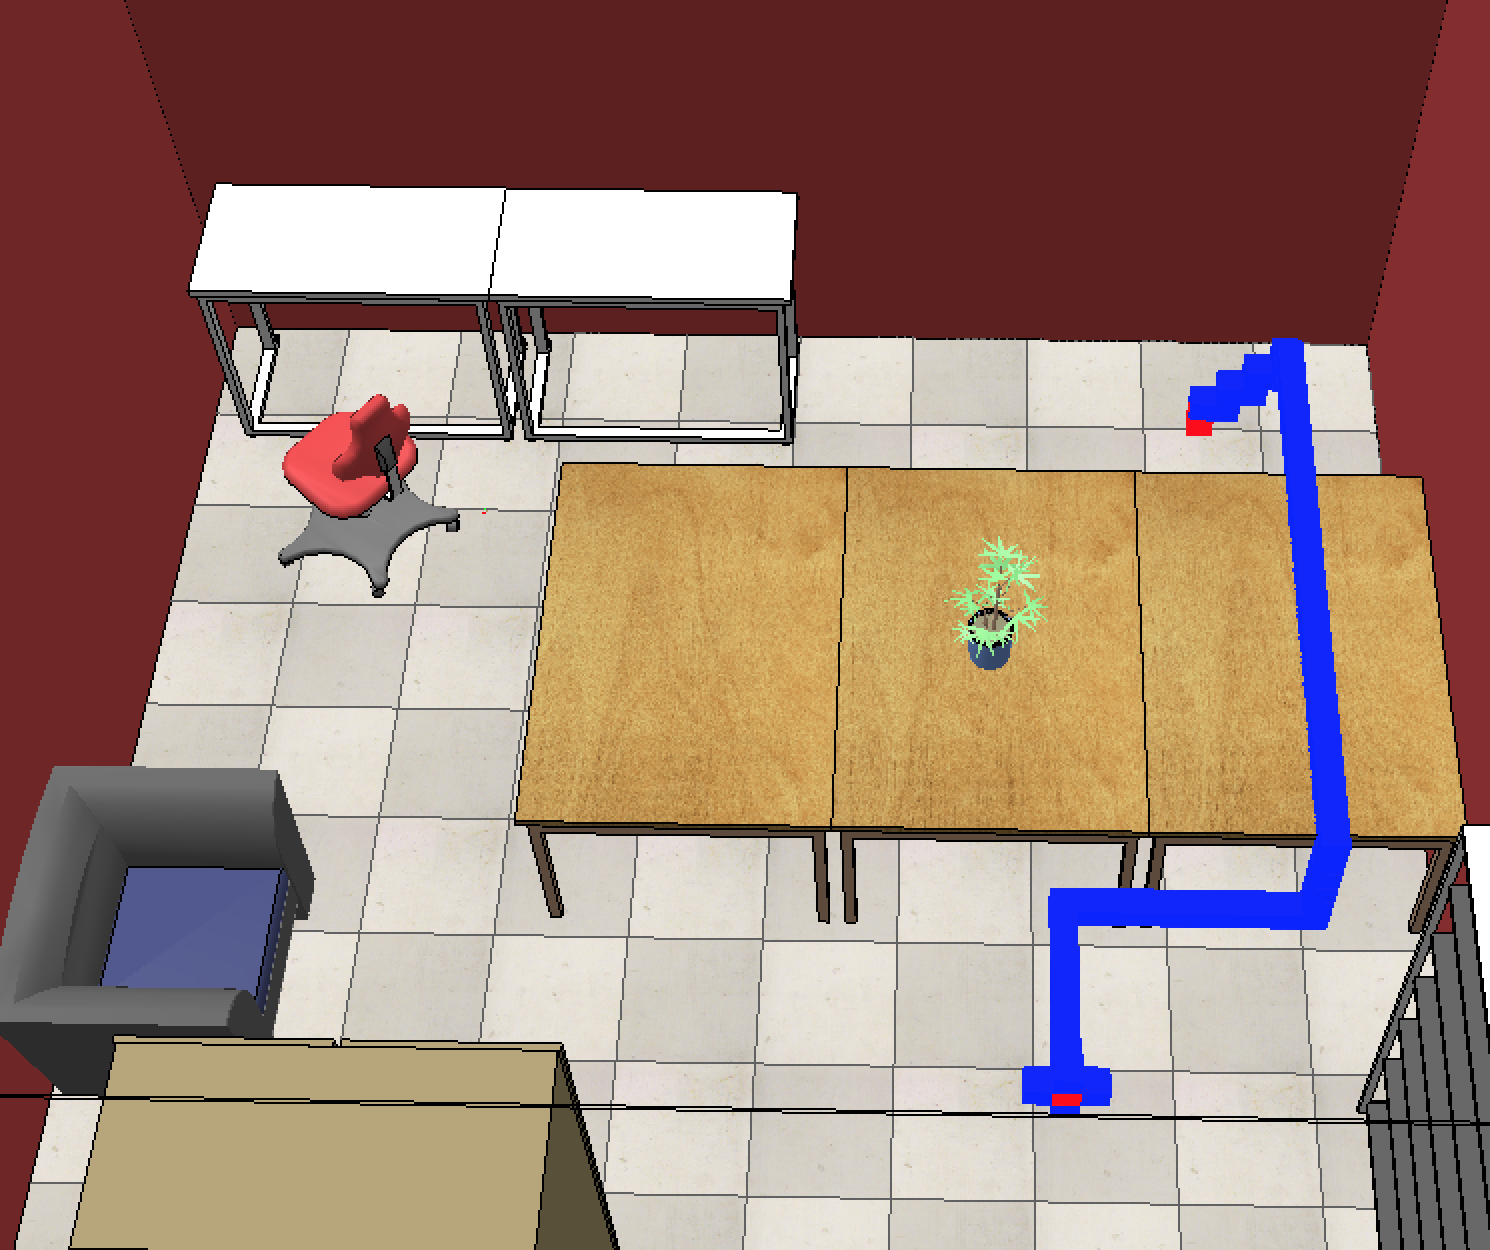
\includegraphics[width=0.9\linewidth]{figures/planned_path.png}
    \caption{This figure illustrates the \textit{room adversarial} environment with an example planning problem (red) and the expanded graph by \phil (blue).}
  \label{fig:room-adv}
\end{wrapfigure}

In our final experiment, we use \phil to plan collision-free paths in a practical drone flight use case within an indoor environment. We built our environment using the CoppeliaSim simulator \cite{coppeliaSim}, and the Ivy framework \cite{lenton2021ivy}. Figure \ref{fig:room-adv}  presents the environment which we refer to as \textit{room adversarial} in Table \ref{tab:table-3}. We discretize the environments into 3D grid graphs of size $50 \times 50 \times 25$, and randomly remove $5$ sub-graphs of size  $5 \times 5 \times 5$ both during training and testing, this way simulating real-life planning scenarios with random obstacles. The hyperparameter configuration and the specific architecture we utilize are equivalent to Section \ref{sec:experiments-grids}, but with $n = 4$. Likewise, the node features are 3D grid coordinates, and the baselines include supervised learning (SL), $h_{euc}$, A*, and BFS, similarly as in Sections \ref{sec:experiments-grids}, \ref{sec:experiments-diversity}. In Table \ref{tab:table-3} we report the ratio of expanded nodes with respect to $h_{euc}$. 

\xhdr{Video demo} We provide a video demonstration of \phil running in \textit{room adversarial}: \url{https://cutt.ly/eniu5ax}.
\begin{table*}[!htb]
\centering
\caption{Results of \phil in the context of planning for indoor UAV flight. \phil outperforms all baselines in both the \textit{room simple} and \textit{room adversarial} environments while remaining close performance-wise to the optimal number of expansions.}
\label{tab:table-3}
\resizebox{0.7\columnwidth}{!}{%

\begin{tabular}{cccccccc|c} \toprule
 \textbf{Dataset}                     & \textbf{SL} &\textbf{A*} & $h_{euc}$ & \textbf{BFS} & \textbf{\sail} & \textbf{BFWS} & \textbf{\phil} & \textbf{Shortest path} \\ \midrule
Room simple   & 1.124 & 76.052  & 1.000 & 291.888 & 0.973 & 1.286 & \textbf{0.785} &0.782                 \\ 
Room adversarial  & 2.022 & 67.215   & 1.000 & 238.768 & 0.944 & 1.583 & \textbf{0.895} & 0.853                  \\ \bottomrule
\end{tabular}
}
\end{table*}

\xhdr{Discussion} As we can observe in Table \ref{tab:table-3}, \phil outperforms all baselines in both environments. Interestingly, \phil expands only approximately $0.3\%$ more nodes in the simple room than least possible and $4.9\%$ more in the adversarial room case. The same figures for the greedy method ($h_{euc}$) are $27.8\%$  and $17.2 \%$, respectively. These results indicate that \phil is capable of learning planning strategies that are close to optimal in both \textit{simple} and \textit{adversarial} graphs, while the performance of naive heuristics degrades.

\subsection{Runtime Analysis}
\label{sec:runtime}
We evaluated the inference runtimes of seven approaches on all datasets in Section~\ref{sec:experiments-grids}. Each approach's runtime was normalized by the number of nodes it visited. The runtime experiments were conducted on a machine with an RTX5000 GPU and an Intel Xeon 5222 CPU.

\begin{figure}[H]
    \centering
    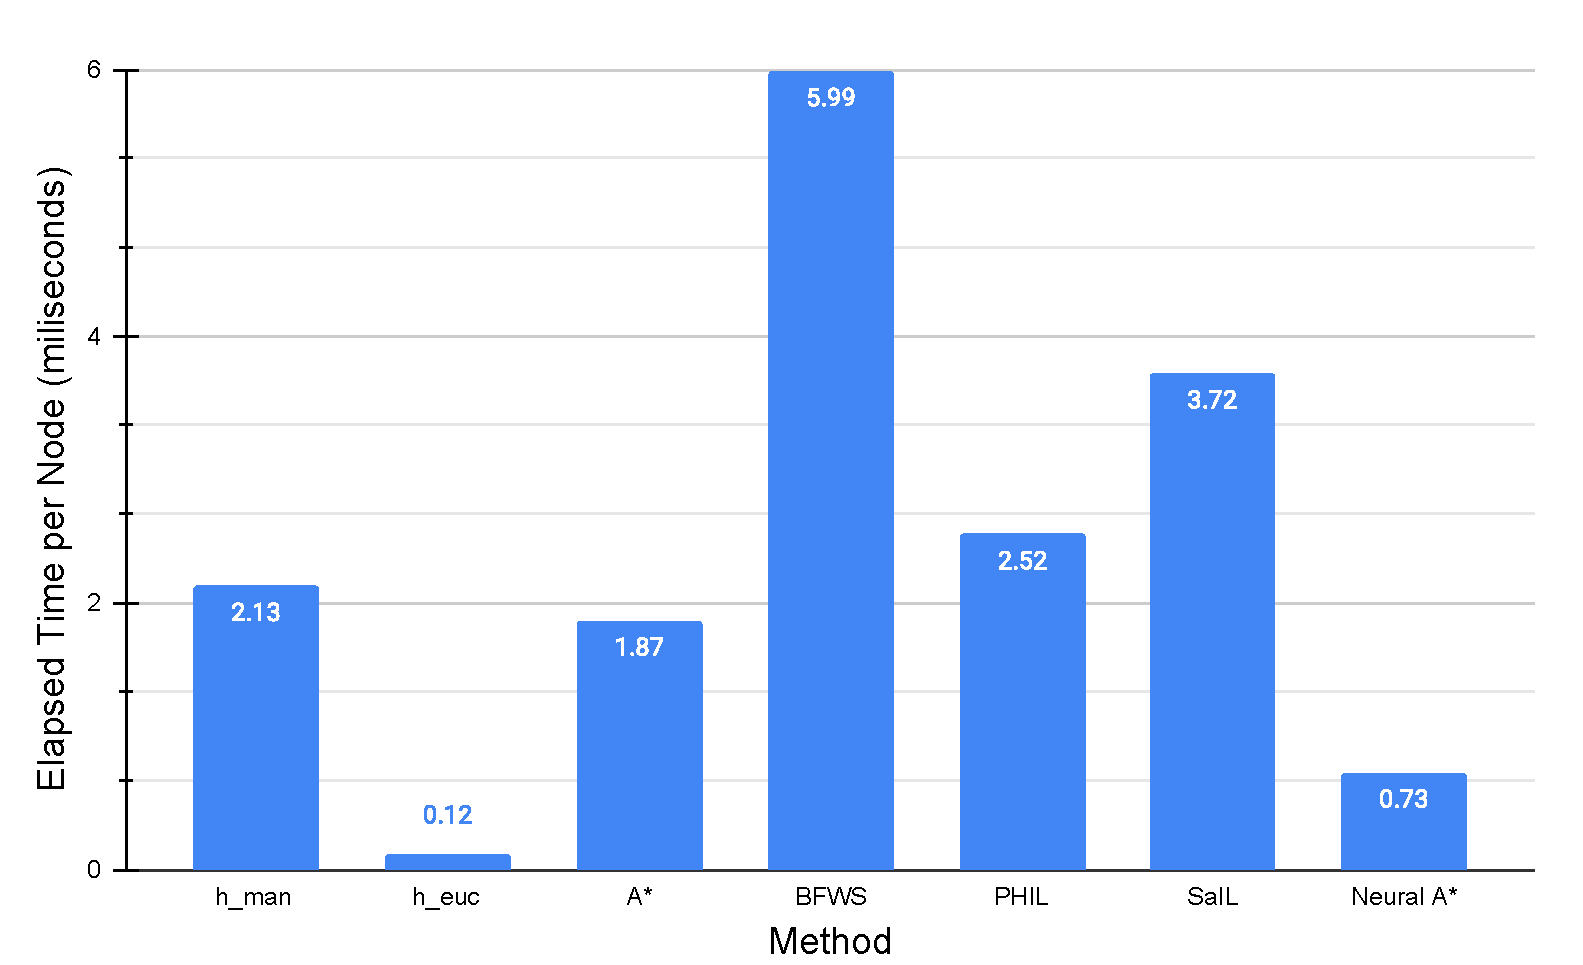
\includegraphics[width=0.9\linewidth]{PHIL/figures/runtime.pdf}
    \caption{Timing experiments on grid search datasets \cite{bhardwaj2017learning}.}
    \label{fig:phil-runtime}
\end{figure}

Figure~\ref{fig:phil-runtime} summarizes the test runtimes of the different approaches. PHIL runs $57.9\%$ faster than BFWS and $32.2\%$ faster than \sail , and not much slower than traditional A* ($34.7\%$) and $h_{man}$ ($18.3\%$). Although Neural A* is $71.0\%$ faster than PHIL due to the fact that it casts the whole search process into matrix operations on images, it cannot be employed in a generic search setting.
\section{Conclusion}

We consider the problem of learning to search for feasible paths in graphs efficiently. We propose a model and a training procedure to learn search heuristics that can be easily deployed across diverse graphs, with tuneable trade-off parameters between constant factors and performance. Our results demonstrate that \phil outperforms current state-of-the-art approaches and can be applied to various graphs with practical use cases.
